%%%%%%%%%%%%%%%%%%%%%%%%%%%%%%%%%%%%%%%%%%%%%%%%%%%%%%%%%%%%%%%%%%%%%%%%%%%%%%%%%
%% Paper M3 -- Target: Software: Practice and Experience (Wiley), Q2
%% Closing the Grace Gap: an adaptive terminationGracePeriodSeconds controller
%% coupling Kubernetes pod termination with BEAM cluster convergence
%% (Horde handoff + libcluster convergence) for zero-loss rolling updates.
%%
%% Template: Wiley New Journal Design v5 (WileyNJDv5.cls). Style chosen via the
%% \documentclass option (AMA = numeric). Do NOT add \bibliographystyle manually;
%% the class sets it from the option.
%%
%% !! COMPILE WITH XeLaTeX (Wiley NJD v5 requires it for its fonts; TeX Live 2022).
%%    latexmk -xelatex main.tex
%%
%% Data: ../data/   Figures: ../figures/   Artifact: ../code/   Plan: ../OUTLINE.md
%%%%%%%%%%%%%%%%%%%%%%%%%%%%%%%%%%%%%%%%%%%%%%%%%%%%%%%%%%%%%%%%%%%%%%%%%%%%%%%%%

\documentclass[AMA,Times1COL]{WileyNJDv5}
% Style options (pick what SP&E mandates): AMA | APA | APS | AMS | Chicago |
%   Harvard | MLA | MPS | Vancouver | WCMS.  Layout: Times1COL | LATO2COL | ...
% AMA = numeric citations (sensible default for a CS systems paper); confirm with SP&E.

\articletype{Original Article}%

\received{Date Month Year}
\revised{Date Month Year}
\accepted{Date Month Year}
\journal{Software: Practice and Experience}
\volume{00}
\copyyear{2026}
\startpage{1}

\usepackage{listings}
\usepackage{algorithm}
\usepackage{algpseudocode}
\usepackage{booktabs}
\usepackage{subcaption}
\usepackage{wrapfig}  % reinstated for the (tall) activity diagram as a text-wrapped figure
% amsthm is loaded by the WileyNJDv5 class. The class already provides a \proposition command, so we
% define a uniquely-named environment for our one lightweight safety proposition (Design section).
\newtheorem{gcprop}{Proposition}

% hyperref and xcolor are already loaded by the WileyNJDv5 class; only set link colours here.
\definecolor{navyblue}{RGB}{0,0,128}
\hypersetup{colorlinks=true,allcolors=navyblue}

\graphicspath{{figures/}{../figures/}}

\lstdefinelanguage{Elixir}{
  morekeywords={def,defp,defmodule,do,end,case,cond,fn,receive,after,when,
    use,import,alias,require,GenServer,Supervisor,Horde,spawn,send,handle_info,
    handle_call,handle_cast,init,true,false,nil},
  sensitive=true, morecomment=[l]{\#}, morestring=[b]"
}
\lstset{basicstyle=\ttfamily\footnotesize, keywordstyle=\bfseries,
  commentstyle=\itshape, showstringspaces=false, breaklines=true,
  frame=lines, numbers=left, numberstyle=\tiny, numbersep=6pt, tabsize=2}

\raggedbottom

\begin{document}

\title{Closing the Grace Gap: An Adaptive Termination-Grace Controller Coupling
Kubernetes Pod Termination with BEAM Cluster Convergence for Zero-Loss Rolling Updates}

\author[1]{Alfa Yohannis}
\author[2]{Alexander Waworuntu}

\authormark{YOHANNIS \textsc{and} WAWORUNTU}
\titlemark{Closing the Grace Gap: Coupling Kubernetes Termination with BEAM Convergence}

\address[1]{\orgdiv{Department of Informatics}, \orgname{Universitas Pradita},
  \orgaddress{\city{Tangerang}, \country{Indonesia}}}
\address[2]{\orgdiv{Department of Informatics}, \orgname{Universitas Multimedia Nusantara},
  \orgaddress{\city{Tangerang}, \country{Indonesia}}}

\corres{Alfa Yohannis, Department of Informatics, Universitas Pradita, Tangerang, Indonesia.
  \email{alfa.ryano@pradita.ac.id}}

%\fundingInfo{}

\abstract[Abstract]{%
Stateful services increasingly run on container orchestrators that add their own recovery on top of
the application runtime's. When such a service is upgraded, or a machine is withdrawn for
maintenance, an instance that is about to be removed must first migrate its in-memory state to
surviving instances and let the cluster settle before it disappears. To bound this shutdown, the
orchestrator grants a fixed, operator-chosen \emph{grace period} and then forcibly terminates the
instance. We argue that a fixed grace period is structurally mismatched to this task: set it too low
and forced termination interrupts the migration, losing state and availability; set it defensively
high and every instance slows the rollout, making upgrades sluggish and resource-hungry. The time
actually required is not a constant---it grows with the amount of state to migrate and with the load
on the cluster---so no single value is right for all instances or all moments. We present a
cross-layer feedback controller that \emph{derives} the grace period at run time from the runtime's
own progress signals rather than guessing it in advance, and that paces the rollout accordingly. We
formalise a safety condition relating the orchestrator's shutdown window to the runtime's migration
and convergence time, provide an open reference implementation on Kubernetes, and evaluate it against
fixed and over-provisioned baselines under fault injection. On a two-node cluster the controller
eliminates the state loss that a fixed 30\,s grace incurs once the handoff outlasts it (40 of 160
stateful processes), while granting only the grace actually needed ($16$--$46$\,s) instead of a
fixed, over-provisioned 300\,s.}

\keywords{Kubernetes, Erlang/BEAM, Elixir/OTP, graceful shutdown, rolling update,
fault tolerance, cross-layer coordination, Horde, libcluster}

\maketitle

%====================================================================
\section{Introduction}\label{sec:intro}

Services built on the Erlang BEAM virtual machine---most visibly through Elixir and the OTP
framework---are organised as large numbers of lightweight processes under supervision trees that
restart failed processes in microseconds. A growing number of these services are deployed on
Kubernetes, which adds a second, coarser tier of fault tolerance: it restarts containers, reschedules
pods, and replaces nodes. The two tiers are complementary, operating at different granularities and
timescales, and stateful BEAM applications routinely rely on both at once: process state that must
survive a pod's disappearance is held in distributed registries such as Horde~\cite{horde} and made
discoverable through cluster-formation libraries such as libcluster~\cite{libcluster}.

The two tiers must nonetheless cooperate at one specific moment: when a pod is deliberately removed.
During a rolling update or a node drain, Kubernetes terminates a pod by sending \texttt{SIGTERM},
optionally running a \texttt{preStop} hook, waiting for a bounded \emph{grace period}
(\texttt{terminationGracePeriodSeconds}), and then sending \texttt{SIGKILL}~\cite{k8sgraceful}.
A stateful BEAM pod must use that window to \emph{hand off} its processes to surviving pods and let
the cluster re-converge (membership stabilises, registries reconcile, singletons re-register) before
it disappears. The grace period therefore acts as a deadline on cross-tier handoff.

The difficulty is that this deadline is a \emph{static constant chosen by the operator at deploy
time}. If it is shorter than the handoff plus convergence time, \texttt{SIGKILL} interrupts the
handoff and state is lost---registered singletons vanish and requests fail until the cluster
re-converges. If it is set defensively high, the cost reappears at the other end: a rolling update
advances only as fast as each pod's grace allows, so an over-long grace makes every deployment slow
and resource-hungry. Crucially, the time actually required is not fixed: it grows with the number of
stateful processes a pod holds, shrinks with the achievable handoff rate, and depends on cluster
convergence time---all of which vary with load. A single constant cannot be simultaneously safe and
efficient, and a fixed \texttt{preStop} sleep is equally blind. This is a cross-layer coordination
gap: the orchestrator owns the deadline, the runtime owns the information that should set it, and
nothing connects them.

We close that gap with a \emph{grace-convergence controller}: a cross-layer feedback loop that
\emph{derives} the grace period at run time from runtime convergence signals rather than guessing it
in advance. A lightweight probe exposes the pod's handoff backlog, its observed handoff rate, and its
membership-convergence state; a Kubernetes operator uses these to compute a per-pod grace period and
to pace the rolling update; and an adaptive \texttt{preStop} hook drains and then blocks precisely
until handoff completes instead of sleeping for a guessed interval. The result is a deadline that is
just long enough to be safe and no longer.

This paper makes the following contributions:
\begin{enumerate}
  \item A \emph{grace-safety invariant} that formalises, across the orchestrator/runtime boundary,
        when a graceful termination is safe (Section~\ref{sec:model}), a policy that provably
        satisfies it under a conservative rate estimate (Proposition~\ref{prop:safety}), and an
        analysis of why both static and over-provisioned grace periods fall short.
  \item The design of a cross-layer grace-convergence controller, decomposed into runtime-agnostic
        roles so that the principle transfers beyond the BEAM (Section~\ref{sec:design}).
  \item A reference implementation as an open artifact---built from libcluster, Horde, a Kubernetes
        operator, and an adaptive \texttt{preStop} hook (Section~\ref{sec:impl}).
  \item An empirical evaluation on Kubernetes against static, over-provisioned, and fixed-sleep
        baselines, measuring state loss, rollout time, adaptivity, controller overhead, scalability
        to a per-node handoff ceiling, behaviour under injected real network latency, fail-safe
        response to faults, and a realistic-workload case study on Phoenix.Presence
        (Section~\ref{sec:eval}).
\end{enumerate}

%====================================================================
\section{Background and Motivation}\label{sec:bg}

\subsection{Pod termination and rolling updates in Kubernetes}\label{sec:bg-k8s}
Kubernetes terminates a pod through a fixed lifecycle~\cite{k8sgraceful}. The pod is marked
\emph{Terminating} and removed from service endpoints; an optional \texttt{preStop} hook runs; the
container receives \texttt{SIGTERM}; and after at most \texttt{terminationGracePeriodSeconds} (default
30\,s) the container is forcibly killed with \texttt{SIGKILL}. The grace period is thus a hard upper
bound on whatever cleanup the application performs after \texttt{SIGTERM}, including any \texttt{preStop}
work. Deliberate removals happen routinely: a \emph{rolling update} replaces pods a few at a time,
bounded by \texttt{maxUnavailable} and \texttt{maxSurge}, and a \emph{node drain} (for maintenance or
scale-down) evicts every pod on a node. In all of these, the grace period governs how long each pod
has to wind down cleanly.

\subsection{Stateful clusters on the BEAM}\label{sec:bg-beam}
A BEAM application is a cluster of nodes (one per pod, typically) whose processes are supervised
intra-node by OTP and discovered inter-node through a membership layer such as
libcluster~\cite{libcluster}, which forms the cluster from Kubernetes endpoints and must
\emph{converge} after any topology change. Stateful work is commonly placed in a distributed
registry and supervisor such as Horde~\cite{horde}, which uses delta-CRDTs so that, when a node
leaves, the processes it owned can be \emph{handed off} and restarted on surviving nodes and
cluster-wide singletons re-registered. Handoff and re-convergence are not instantaneous: their
duration grows with the number of processes a departing node holds and with the time the membership
and CRDT state take to stabilise. Practitioners report these graceful-shutdown and handoff concerns
as first-order issues when running such systems on Kubernetes~\cite{souza2024dependable}.

\subsection{The grace gap}\label{sec:bg-gap}
Combining the two, a terminating stateful pod must complete drain, handoff, and re-convergence
\emph{within} its grace period, or \texttt{SIGKILL} will cut it off mid-handoff
(Figure~\ref{fig:problem}). Consider an illustrative deployment in which a pod hosts a few hundred
stateful processes and, under the cluster's current load, handoff plus convergence takes about
45\,s. With the default grace of 30\,s, \texttt{SIGKILL} arrives while roughly 150 processes are
still in flight: their state is lost and the singletons they hosted are unavailable until the cluster
re-converges. Raising the grace to, say, 300\,s removes the loss but makes every pod in a rolling
update wait up to five minutes before the next can proceed. Because the required time tracks load,
neither constant is right in general---motivating a grace period that is computed from the runtime's
actual state rather than fixed in advance.

\begin{figure}[t]
  \centering
  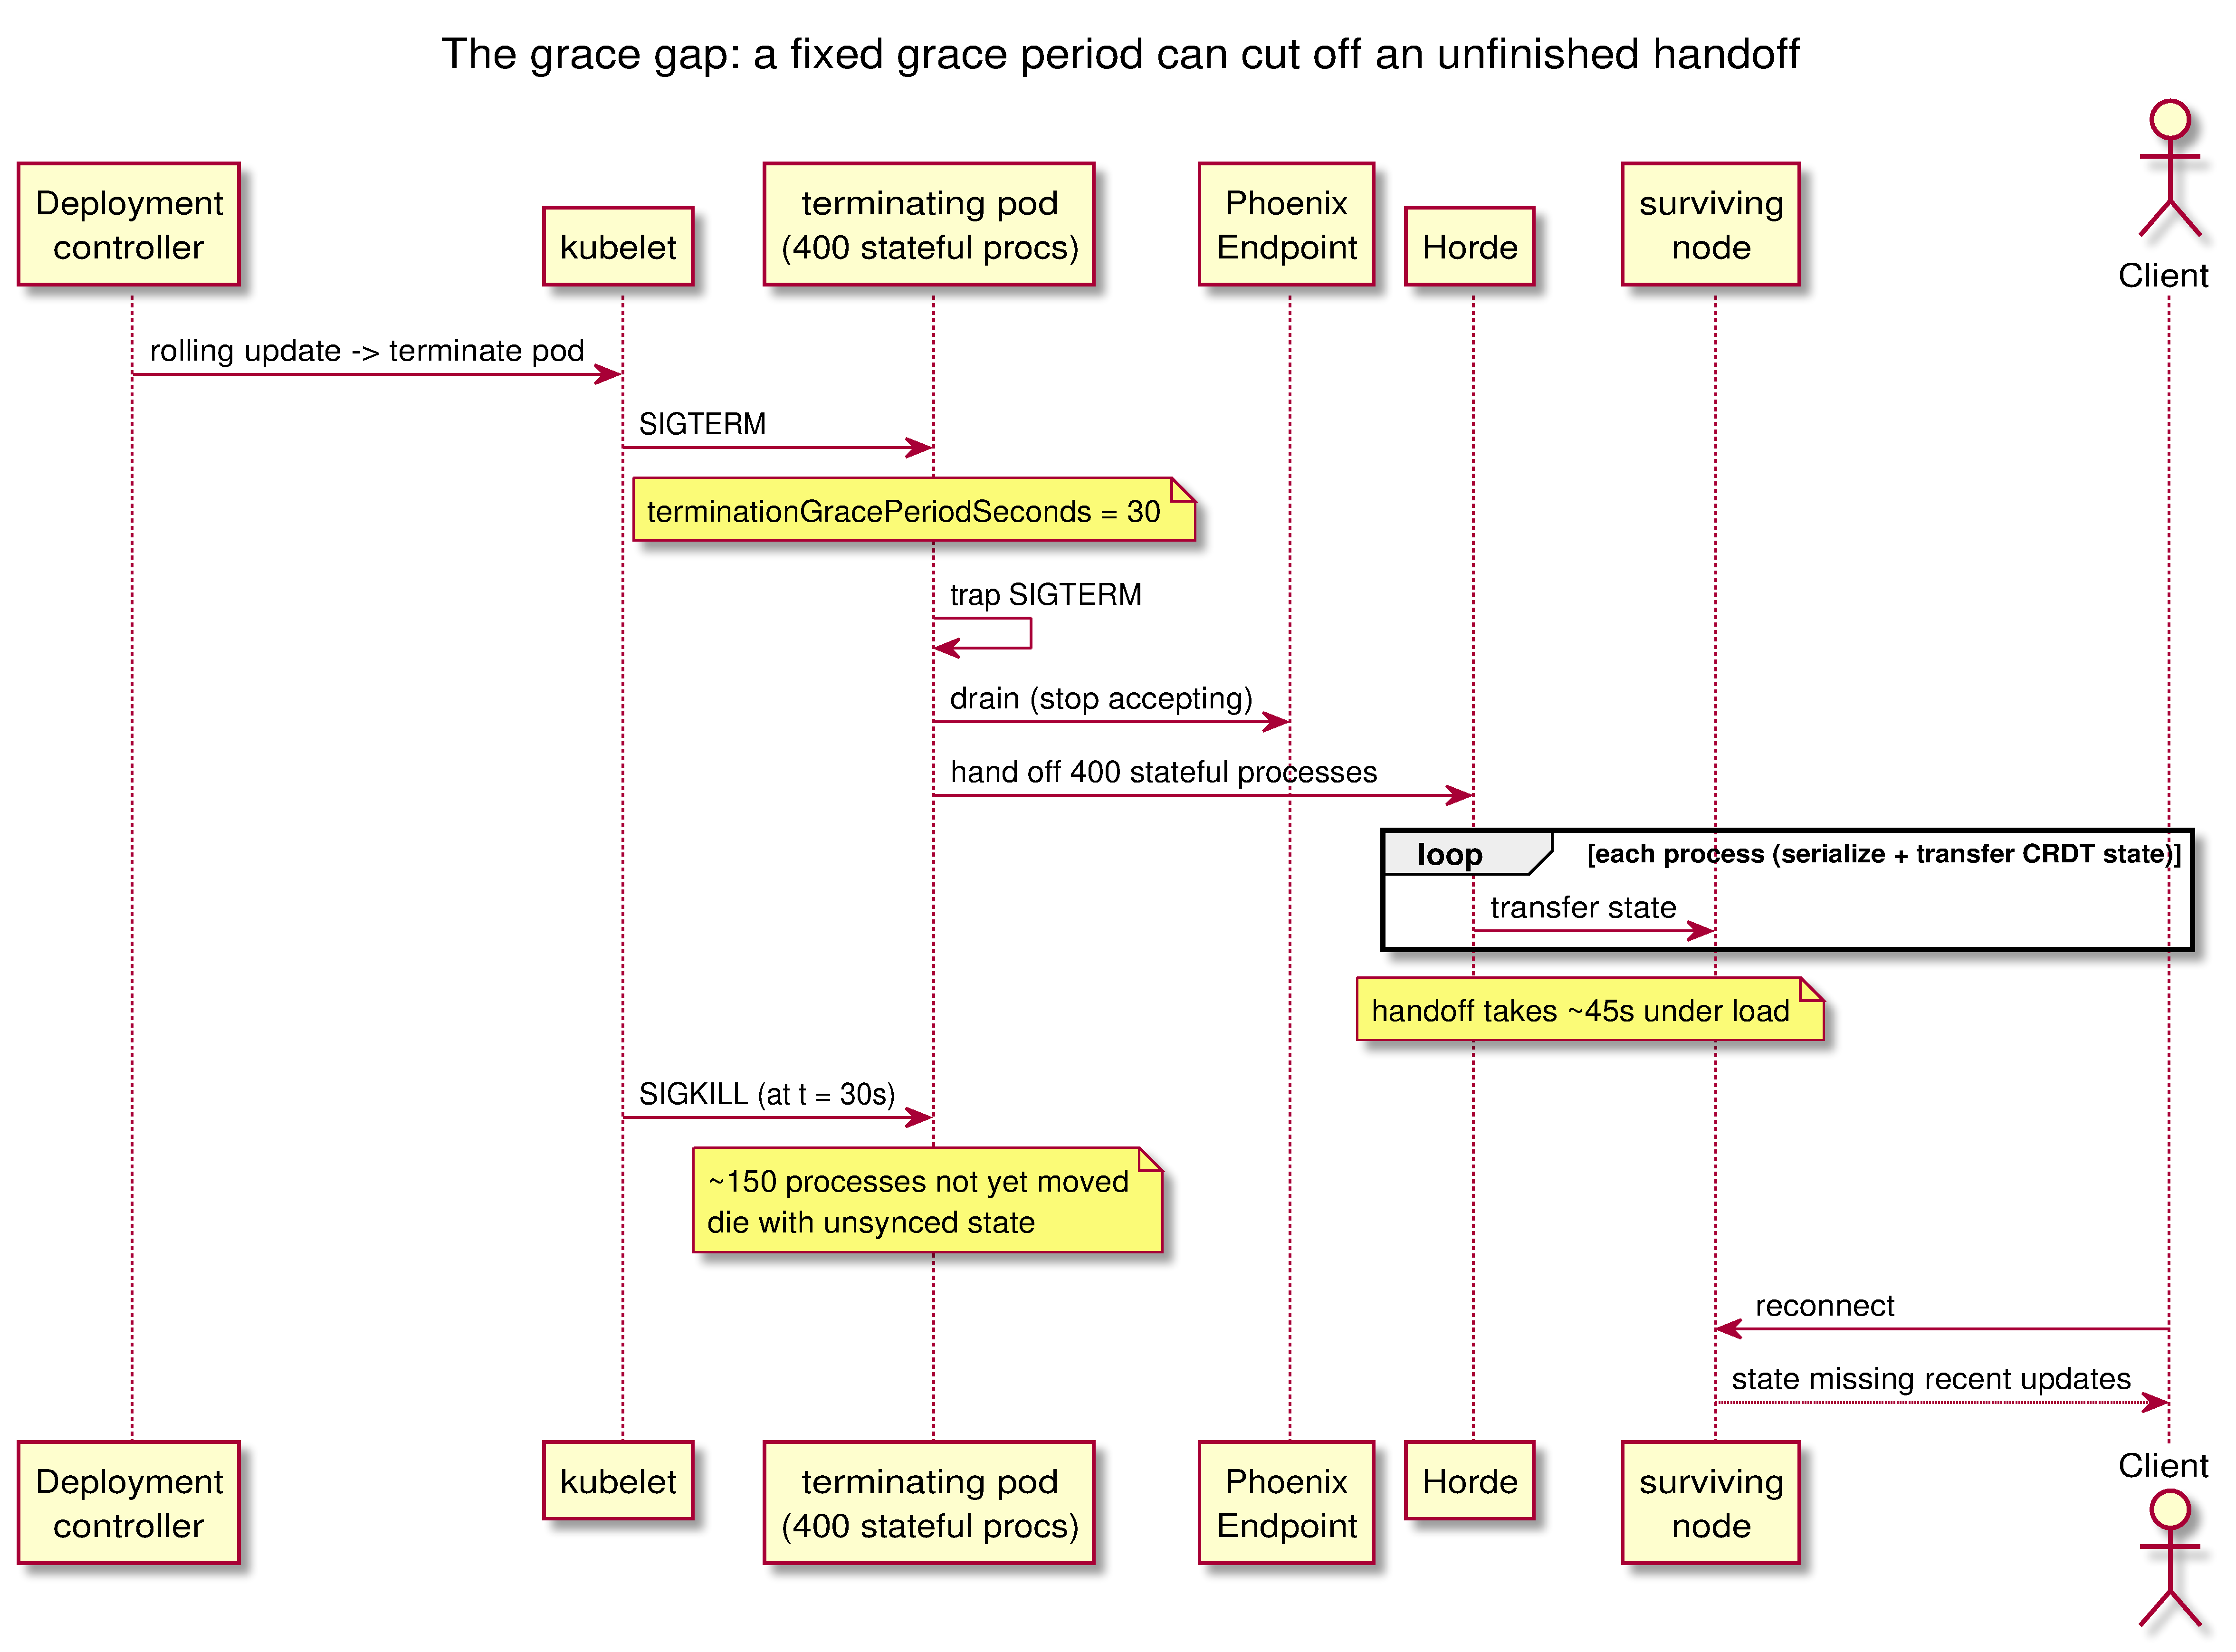
\includegraphics[width=\linewidth]{grace-gap-problem.pdf}
  \caption{The grace gap (illustrative scenario): a fixed 30\,s grace period forces \texttt{SIGKILL}
  before an $\sim$45\,s handoff completes, so processes still in flight are killed and their recent
  state is lost until the cluster re-converges. The scenario is illustrative.}\label{fig:problem}
\end{figure}

\subsection{Why current approaches fall short}\label{sec:bg-existing}
Return to the scenario of Section~\ref{sec:bg-gap} (Figure~\ref{fig:problem}), where a
$\sim$45\,s handoff is severed by a 30\,s grace. A team facing this can reach for several well-known
options, but none closes the gap: each acts on only \emph{one side} of the orchestrator/runtime
boundary, whereas the gap is precisely a \emph{cross-layer} mismatch.

\paragraph{Enlarging the grace period.} The reflex is to raise
\texttt{terminationGracePeriodSeconds}~\cite{k8sgraceful} to a generous worst case. This merely
trades one cost for another: because a rolling update advances no faster than the grace each pod
actually consumes, an over-long grace inflates every deployment and ties up capacity. It is also
still a fixed guess---a load spike that pushes handoff beyond the assumed worst case truncates state
anyway (the 45\,s of Figure~\ref{fig:problem} could just as easily be 90\,s)---and it cannot shrink
when load is light, so the common case keeps paying for the rare one.

\paragraph{A fixed \texttt{preStop} sleep.} Sleeping for a constant interval in the
\texttt{preStop} hook~\cite{k8sgraceful} is the same blind guess in different clothing: it neither
observes how much handoff remains nor guarantees it finishes. Too long wastes the window; too short
still lets \texttt{SIGKILL} cut in.

\paragraph{Readiness and liveness probes.} Probes~\cite{k8sgraceful} gate traffic and trigger
restarts from a per-pod health signal. They are orthogonal to termination: they cannot lengthen,
shorten, or otherwise coordinate the kill deadline, so they say nothing about whether a departing pod
has finished the handoff of Figure~\ref{fig:problem}.

\paragraph{PodDisruptionBudgets.} A PDB~\cite{k8sPDB} limits how many pods may be voluntarily
disrupted at once. That is an availability \emph{count} constraint, not a per-pod completion check:
it does not know whether a given pod has drained its state, and it never extends that pod's
grace---so a pod can still be \texttt{SIGKILL}ed mid-handoff while the budget is satisfied.

\paragraph{Application-level graceful shutdown alone.} The application can trap \texttt{SIGTERM},
stop accepting work, and hand off correctly---yet it is racing a fixed external deadline it has no
way to influence. When handoff legitimately needs longer than the configured grace (as in
Figure~\ref{fig:problem}), doing everything right internally does not help: the orchestrator kills it
regardless.

\paragraph{Runtime-native coordinated shutdown.} Actor runtimes offer phased shutdown---Akka's
\emph{CoordinatedShutdown}~\cite{akkacoordinated} and Orleans' graceful deactivation~\cite{orleans}
(Section~\ref{sec:related}). These run ordered phases with \emph{configured} per-phase timeouts that
live inside the runtime and are never communicated to the orchestrator's grace period. The phases are
better-structured guesses, but they are still guesses, and the cross-layer deadline stays uninformed.

\paragraph{Speeding up or sharding the handoff.} Reducing $|H_p|$ or raising the handoff rate $\rho$
shrinks the time needed and certainly helps, but it is a mitigation, not a fix: the required time
still varies with load, and the deadline is still set without reference to it.

\paragraph{Cross-layer coordination exists---but for other concerns.} A body of work \emph{does} cross
the boundary, which makes the specific omission sharper. Signal-based health monitoring derives a
pod's Kubernetes health from runtime state instead of polling it~\cite{roberts2025}, and actor
frameworks expose comparable runtime health to the orchestrator~\cite{akkaHealth}---but this
coordinates the \emph{health probe}, not the termination deadline. Leases and split-brain resolvers
coordinate cluster \emph{membership and quorum} across the two layers~\cite{akkaLease,akkaSBR};
autonomic and operator-driven controllers manage \emph{placement and lifecycle}~\cite{kephart2003,
meliani2025proactive}; rollback-recovery and checkpointing \emph{preserve state} for restoration
elsewhere~\cite{elnozahy2002}; and deployment-time optimisation plans placement under fault-tolerance
and latency constraints~\cite{ucc23,gustafsson2025rtilience}. Each is genuinely cross-layer, yet none
couples the termination grace period to the runtime's handoff and convergence progress---so in
Figure~\ref{fig:problem} the pod is still killed at 30\,s with its handoff unfinished.

\medskip\noindent
What unites these is one structural fact: the \emph{information} needed to choose a correct
deadline---the runtime's handoff backlog, achievable rate, and convergence state---lives in the
runtime, while the \emph{control} that enforces the deadline---the grace period and the rollout
pace---lives in the orchestrator, and nothing carries the former to the latter. Every option above
either freezes a constant ahead of time or operates within
a single layer; none establishes a feedback path across the boundary (Table~\ref{tab:existing}).
Building that path is exactly what our controller does (Section~\ref{sec:design}).

\begin{table}[t]
\centering
\caption{Standard responses to the grace gap and why each fails to close it: every one acts within a
single layer, so none derives the deadline from runtime state.}\label{tab:existing}
\begin{tabular}{@{}p{0.30\linewidth}p{0.15\linewidth}p{0.47\linewidth}@{}}
\toprule
\textbf{Approach} & \textbf{Acts on} & \textbf{Why it cannot close the grace gap} \\
\midrule
Large static grace (over-provision)~\cite{k8sgraceful} & orchestrator & fixed guess; inflates every rollout; still truncates under heavier-than-assumed load \\
Fixed \texttt{preStop} sleep~\cite{k8sgraceful} & runtime hook & blind constant; ignores actual handoff progress \\
Readiness / liveness probes~\cite{k8sgraceful} & orchestrator & gate traffic/restart per pod; do not set or extend the kill deadline \\
PodDisruptionBudget~\cite{k8sPDB} & orchestrator & limits disrupted pod \emph{count}, not handoff completion; never extends grace \\
App-level graceful shutdown alone & runtime & races a fixed external deadline it cannot influence \\
Runtime-native coordinated shutdown~\cite{akkacoordinated,orleans} & runtime & configured internal timeouts; not fed to the orchestrator grace \\
Signal-based health / lease / autonomic lifecycle~\cite{roberts2025,akkaLease,kephart2003} & both layers & genuinely cross-layer, but coordinate health/quorum/placement---not the grace deadline \\
Faster / sharded handoff~\cite{elnozahy2002} & runtime & mitigation only; required time still varies, deadline still blind \\
\bottomrule
\end{tabular}
\end{table}

%====================================================================
\section{System Model and Problem Definition}\label{sec:model}

\subsection{Model}\label{sec:model-model}
We consider a BEAM application running as a Kubernetes \emph{Deployment} of $n$ pods, each pod a
cluster node. When a pod $p$ is selected for termination it must perform three actions before it can
disappear safely:
\begin{enumerate}
  \item \emph{drain} in-flight requests, taking time $T_d(p)$;
  \item \emph{hand off} the set $H_p$ of stateful processes it owns to surviving pods, at an
        achievable rate $\rho(p)$ processes per second, taking time $|H_p|/\rho(p)$; and
  \item allow the cluster to \emph{re-converge}---membership stabilises and registries reconcile---
        taking time $T_c$.
\end{enumerate}
The orchestrator grants the pod a grace period $g$: it sends \texttt{SIGTERM} at time $0$ and
\texttt{SIGKILL} at time $g$. Of these quantities, $|H_p|$, $\rho(p)$, $T_d(p)$ and $T_c$ are
properties of the \emph{runtime under its current load}, whereas $g$ is set by the \emph{orchestrator};
in standard practice $g$ is a single constant configured at deploy time and shared by all pods.

\subsection{Grace-safety invariant}\label{sec:model-invariant}
A termination is \emph{safe} (no handoff is truncated, no state is lost) only if the grace period
covers drain, handoff, and convergence:
\begin{equation}\label{eq:invariant}
  g \;\ge\; T_d(p) \;+\; \frac{|H_p|}{\rho(p)} \;+\; T_c .
\end{equation}
The right-hand side is load-dependent and time-varying: it rises as a pod accumulates stateful
processes ($|H_p|\!\uparrow$), as contention lowers the handoff rate ($\rho\!\downarrow$), or as a
larger or busier cluster takes longer to converge ($T_c\!\uparrow$).

\subsection{Why a constant fails}\label{sec:model-constant}
A small static grace $g_0$ (e.g.\ the 30\,s default) violates Equation~\eqref{eq:invariant} whenever
the load term $|H_p|/\rho(p)$ is large, producing exactly the truncated-handoff loss of
Section~\ref{sec:bg-gap}. Over-provisioning ($g_0$ set to a large worst-case, e.g.\ 300\,s) restores
safety but is pessimal for throughput: in a rolling update the wall-clock time is bounded below by the
sum of the grace periods actually waited, so a grace far larger than needed directly inflates
deployment time. The objective is therefore to choose, \emph{per pod and per termination}, the
smallest $g$ that still satisfies Equation~\eqref{eq:invariant}:
\begin{equation}\label{eq:objective}
  g^\star(p) \;=\; T_d(p) \;+\; \frac{|H_p|}{\rho(p)} \;+\; T_c .
\end{equation}
Since the right-hand side is known only to the runtime and only at termination time, achieving
$g \approx g^\star$ requires feeding runtime state across the boundary to the orchestrator---the
controller of Section~\ref{sec:design}. We add a safety margin and bounds to
Equation~\eqref{eq:objective} in the design rather than assume the terms are known exactly.

%====================================================================
% Reader-facing title carries NO internal label. (Internally this is mechanism M3
% from the companion report; never surface "M3" to reviewers -- they don't know it.)
\section{Design of the Grace-Convergence Controller}\label{sec:design}
\subsection{Overview}\label{sec:design-overview}


% Terminology convention: describe the mechanism by ROLE (runtime-agnostic) and
% bind each role to a concrete component (Section~\ref{sec:impl}). Standard OS/
% orchestrator terms (SIGTERM, grace period, rolling update, readiness probe) are
% kept as-is. The role vocabulary makes the cross-layer principle portable and
% sets up the comparison with other actor runtimes (Section~\ref{sec:related}).

We describe the design in terms of \emph{roles}---runtime-agnostic
responsibilities---and defer the concrete components that realise each role to
Section~\ref{sec:impl}. Standard operating-system and orchestrator terms
(\texttt{SIGTERM}, the \emph{grace period} \texttt{terminationGracePeriodSeconds},
\emph{rolling update}, \emph{readiness probe}) are used unchanged. Table~\ref{tab:roles}
fixes the role vocabulary and its mapping to our reference implementation; the same
vocabulary lets us compare with other actor runtimes in Section~\ref{sec:related}.

\begin{table}[t]
\centering
\caption{Roles in the mechanism and the concrete components that realise them.
Roles are runtime-agnostic; the rightmost column is specific to our BEAM/Kubernetes
reference implementation (Section~\ref{sec:impl}).}\label{tab:roles}
\begin{tabular}{@{}p{0.30\linewidth}p{0.40\linewidth}p{0.22\linewidth}@{}}
\toprule
\textbf{Role} & \textbf{Responsibility} & \textbf{Component} \\
\midrule
Membership layer & Form the runtime cluster; signal membership convergence & libcluster \\
Registry \& handoff layer & Hold stateful processes; hand them off on shutdown & Horde (delta-CRDT) \\
Convergence probe & Expose handoff backlog, observed handoff rate $\rho$, convergence state & app endpoint \\
Adaptive termination hook & On \texttt{SIGTERM}: drain, then block until handoff completes (not a fixed sleep) & preStop hook \\
Coordinator (operator) & Watch pods; compute and patch the grace period; pace \texttt{maxUnavailable} & Bonny operator \\
Grace-convergence controller \emph{(our contribution)} & Close the loop: set grace $g=f(\text{backlog},\rho,T_c)$ from runtime signals & --- (new) \\
\bottomrule
\end{tabular}
\end{table}


The controller turns Equation~\eqref{eq:objective} into a feedback loop that spans the
orchestrator/runtime boundary. Three roles cooperate (Table~\ref{tab:roles}): a
\emph{convergence probe} exposes the runtime quantities of Section~\ref{sec:model}; the
\emph{coordinator} reads them and sets a per-pod grace period while pacing the rolling update; and
an \emph{adaptive termination hook} ensures the pod actually uses the granted window to finish
handoff instead of sleeping for a guessed interval. Figure~\ref{fig:seq} shows the message flow for a
single termination and Figure~\ref{fig:act} the control loop.

\begin{figure}[t]
  \centering
  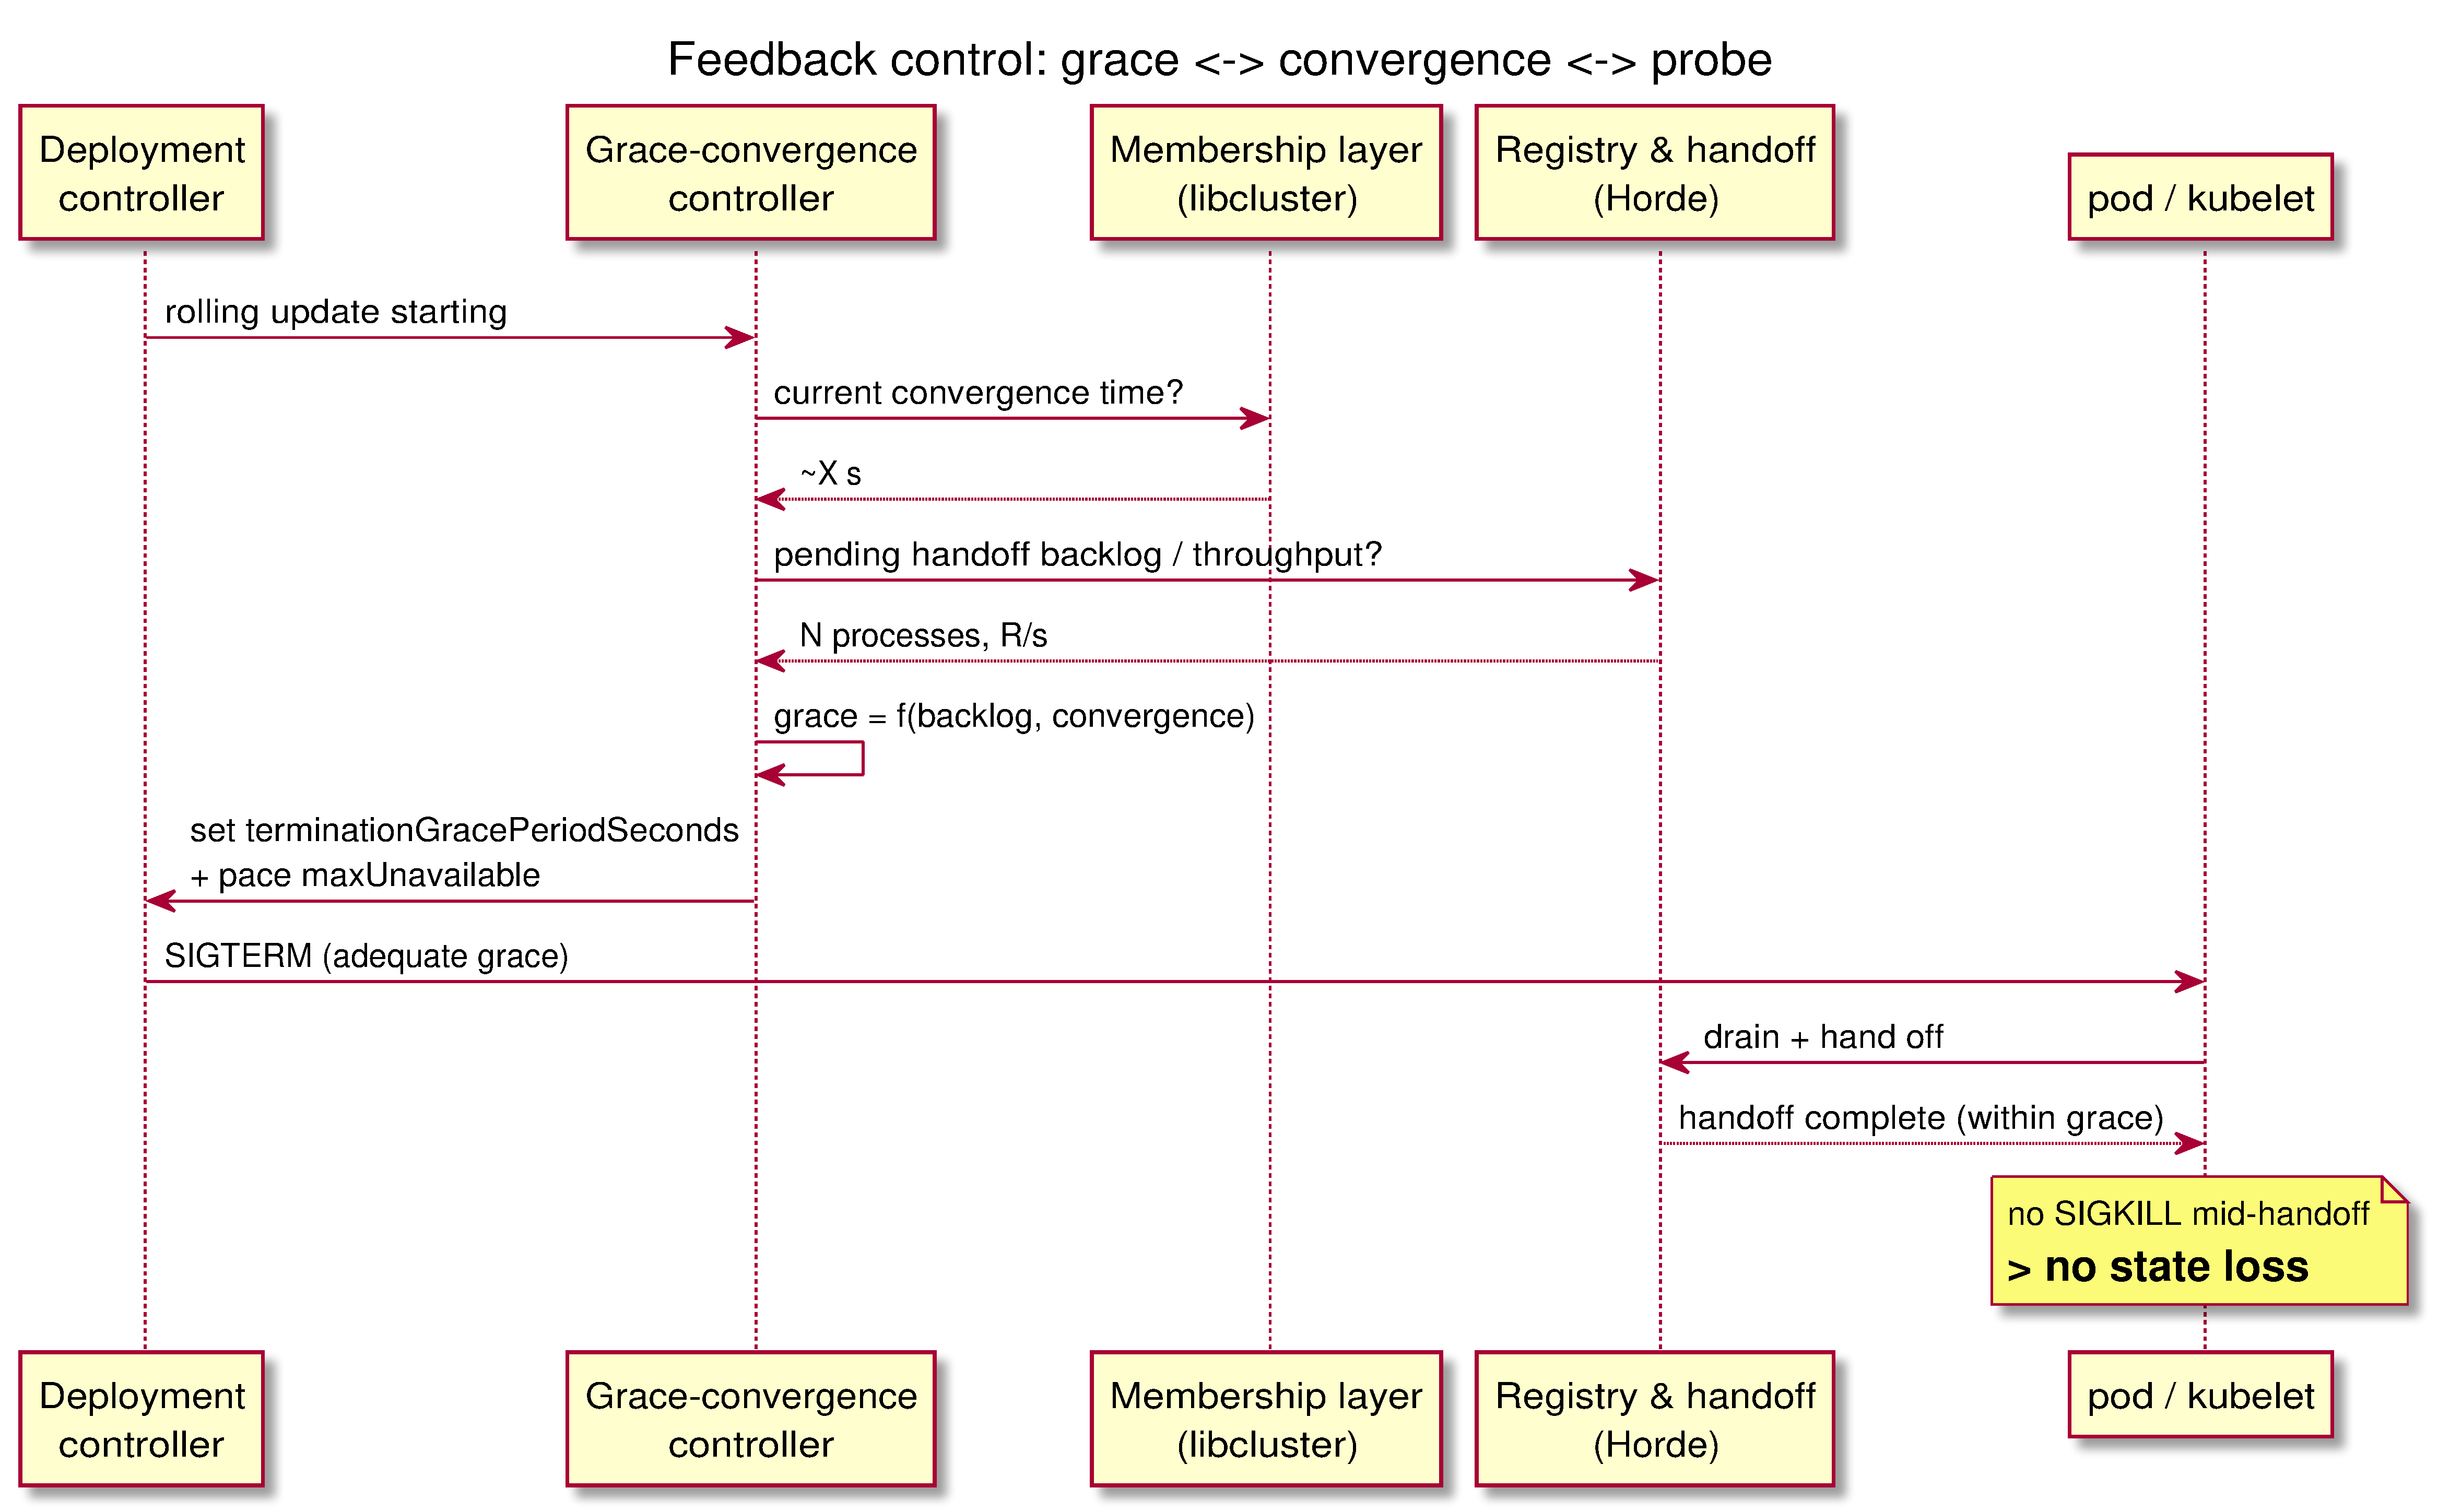
\includegraphics[width=\linewidth]{grace-convergence-sequence.pdf}
  \caption{Message flow for one termination: before \texttt{SIGTERM}, the coordinator queries the
  membership and handoff layers, derives an adequate grace period, and paces the rollout, so the
  handoff completes before \texttt{SIGKILL}.}\label{fig:seq}
\end{figure}

\subsection{Convergence probe}\label{sec:design-probe}

\setlength{\columnsep}{16pt}% gap between the wrapped figure (image AND caption) and body text
\begin{wrapfigure}{r}{0.34\linewidth}
  \centering
  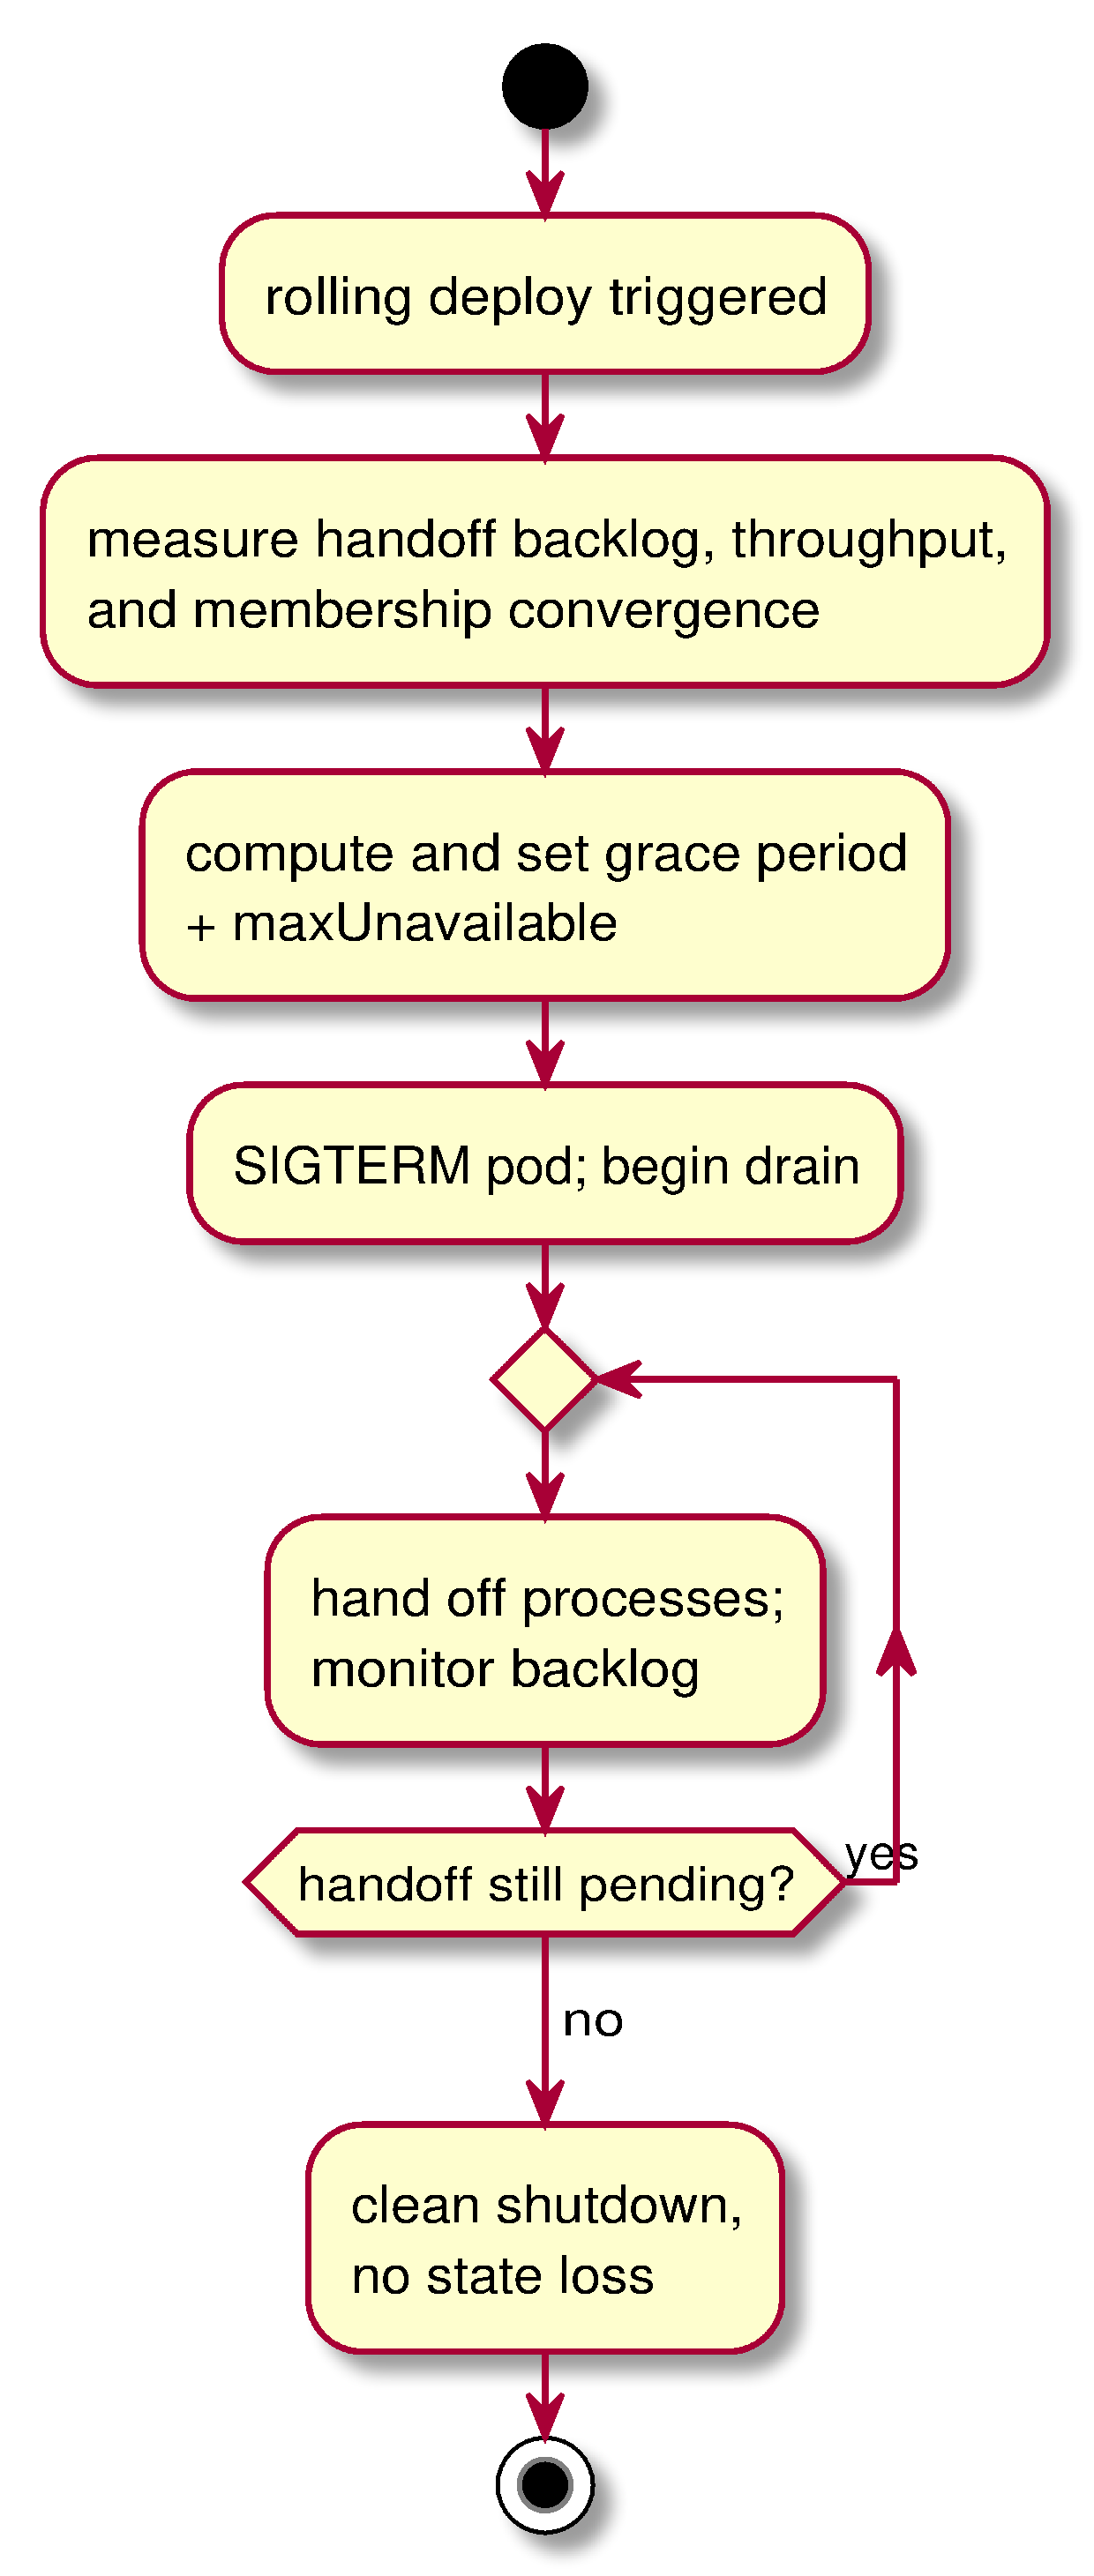
\includegraphics[width=\linewidth]{grace-convergence-activity.pdf}
  \caption{The control loop: measure runtime state, size the grace period and the rollout pace, then
  drain and hand off, repeating while handoff is still pending, until a clean shutdown.}\label{fig:act}
\end{wrapfigure}
\setlength{\columnsep}{10pt}%
Each pod exposes a lightweight endpoint reporting (i) its current handoff backlog $B_p$ (the number of
stateful processes it would need to hand off), (ii) a smoothed estimate of the achievable handoff rate
$\rho_p$, and (iii) the membership layer's convergence state and a recent estimate of $T_c$. The rate
is smoothed with an exponentially weighted moving average over recent handoff activity so that a
transient stall does not produce a wildly large estimate. The probe is read-only and side-effect free,
so it can be polled by the coordinator without perturbing the runtime.

\subsection{Coordinator and grace computation}\label{sec:design-coord}
The coordinator is a Kubernetes operator that watches Deployments and, when a rolling update or drain
is about to remove a pod, reads that pod's probe and computes a grace period from
Equation~\eqref{eq:objective} with a safety margin $\sigma$ and bounds (Algorithm~\ref{alg:grace}).
The lower bound $g_{\min}$ preserves baseline drain behaviour; the upper bound $g_{\max}$ caps the wait
so a misbehaving pod cannot stall a rollout indefinitely. The coordinator writes the computed value to
the pod's \texttt{terminationGracePeriodSeconds} and \emph{paces} the update: it admits the next pod
into the disruption only once the current pod reports handoff complete (or its grace elapses), so the
rollout runs as fast as handoff allows and no faster.

\begin{algorithm}[t]
\caption{Adaptive grace computation and rollout pacing (coordinator side).}\label{alg:grace}
\begin{algorithmic}[1]
\Require margin $\sigma$, bounds $g_{\min}, g_{\max}$
\Procedure{OnTerminate}{pod $p$}
  \State $(B_p,\ \rho_p,\ T_c,\ T_d) \gets \Call{ReadProbe}{p}$
  \State $g^\star \gets T_d + B_p/\rho_p + T_c + \sigma$ \Comment{Eq.~\eqref{eq:objective} with margin}
  \State $g \gets \min\big(g_{\max},\ \max(g_{\min},\ g^\star)\big)$ \Comment{clamp to bounds}
  \State \Call{SetGracePeriod}{$p, g$}
  \State \Call{StartTermination}{$p$} \Comment{kubelet sends \texttt{SIGTERM}}
  \State \textbf{wait until} \Call{HandoffComplete}{$p$} \textbf{or} $g$ elapsed
  \State \Call{AdmitNextPod}{} \Comment{pace \texttt{maxUnavailable}}
\EndProcedure
\end{algorithmic}
\end{algorithm}



\subsection{Adaptive termination hook}\label{sec:design-hook}

A granted grace period is useful only if the pod spends it finishing handoff rather than sleeping for
a fixed interval (a common but blind \texttt{preStop} idiom). On \texttt{SIGTERM} the hook drains
in-flight work and then blocks while handoff is pending, returning as soon as the backlog is cleared
(Figure~\ref{fig:act}). Because the coordinator has already sized the grace period to cover the
expected handoff, this block almost always returns well before $g_{\max}$; the cap exists only as a
backstop.

\subsection{Fail-safes and scope}\label{sec:design-failsafe}

The controller is designed to degrade safely. If a probe is unavailable or returns implausible values,
the coordinator falls back to a configured conservative grace (a default-safe, not default-fast,
choice). The bounds $g_{\min}$ and $g_{\max}$ guarantee progress in both directions. Grace assignment
and pacing are idempotent, so a coordinator restart during a rollout does not corrupt the update.
The mechanism addresses \emph{voluntary} disruptions (rolling updates, drains, scale-down); sudden,
non-graceful node death gives no grace window and is out of scope here. Coordinating disruption
\emph{budgets} with cluster quorum is a complementary, orthogonal mechanism that we do not address in
this paper.

\subsection{Safety guarantee}\label{sec:design-safety}

The policy is constructed so that, under a conservative rate estimate, it provably satisfies the
grace-safety invariant of Equation~\eqref{eq:invariant}.

\begin{gcprop}[Termination safety]\label{prop:safety}
Let a pod terminate with drain time $T_d\ge 0$, convergence time $T_c\ge 0$, backlog $H_p$, and
achievable handoff rate $\rho(p)>0$, and let the coordinator use rate estimate $\hat\rho>0$ and
margin $\sigma\ge 0$. If \emph{(i)}~$\hat\rho\le\rho(p)$ and \emph{(ii)}~the unclamped grace
$g^\star=T_d+|H_p|/\hat\rho+T_c+\sigma$ satisfies $g^\star\le g_{\max}$, then the grace $g$ produced by
Algorithm~\ref{alg:grace} satisfies Equation~\eqref{eq:invariant}, and no stateful process is lost to
a truncated handoff.
\end{gcprop}

\begin{proof}
Algorithm~\ref{alg:grace} sets $g=\min\!\big(g_{\max},\max(g_{\min},g^\star)\big)$. By hypothesis~(ii),
$g^\star\le g_{\max}$, so $g=\max(g_{\min},g^\star)\ge g^\star$. By hypothesis~(i),
$\hat\rho\le\rho(p)$, hence $|H_p|/\hat\rho\ge|H_p|/\rho(p)$. Combining,
\[
  g\ \ge\ g^\star\ =\ T_d+\frac{|H_p|}{\hat\rho}+T_c+\sigma
   \ \ge\ T_d+\frac{|H_p|}{\rho(p)}+T_c ,
\]
the last inequality dropping $\sigma\ge 0$. The right-hand side is exactly the invariant, so the
grace window covers drain, handoff, and convergence and the handoff completes before \texttt{SIGKILL}.
\end{proof}

The two hypotheses are precisely the controller's design posture and delimit how it can fail.
Hypothesis~(i) is enforced by biasing the estimate downward and by the default-safe fallback
(Section~\ref{sec:design-failsafe}); violating it---an over-optimistic rate---lets the policy
under-provision, the sensitivity quantified in RQ5. Hypothesis~(ii) fails only when the genuine
requirement exceeds the cap $g_{\max}$; that is the per-node ceiling characterised in RQ6, mitigated
by bounding per-pod backlog and scaling horizontally. Within these bounds safety holds by
construction, and the empirical check of Section~\ref{sec:eval} (Figure~\ref{fig:invariant}) confirms
the granted grace never falls below the realised handoff time.

%====================================================================
\section{Implementation}\label{sec:impl}
We implement the controller as an open-source Elixir/OTP application of about 660 lines.\footnote{Full
source in \texttt{code/}; a reproduction guide is in Appendix~\ref{app:repro} and an archival snapshot
in \texttt{zenodo/}.} It binds the runtime-agnostic roles of Section~\ref{sec:design}
(Table~\ref{tab:roles}) to concrete components: cluster \emph{membership} to libcluster, cluster-wide
process \emph{identity} and state \emph{handoff} to Horde, the per-pod \emph{probe} and drain endpoint
to Bandit/Plug, and the \emph{coordinator} to a Kubernetes operator. A single release image runs in
two roles, selected by the \texttt{GRACE\_ROLE} environment variable.

\subsection{Stateful workload, identity, and handoff}\label{sec:impl-handoff}
Each stateful unit is a \texttt{GenServer} holding in-memory state. Workers are \emph{hosted} by a
node-local \texttt{DynamicSupervisor} but registered for \emph{identity} in a cluster-wide
\texttt{Horde.Registry} (a $\delta$-CRDT). We deliberately separate hosting from identity: Horde's
distributed supervisor restarts a process at its own ring placement, which can re-home it \emph{back
onto the leaving node}; by hosting locally and using Horde only for lookup, the handoff controls
placement explicitly. A drain reads each worker's state, terminates the local process, and re-creates
it on a chosen survivor. Because the just-killed worker's registry entry can linger briefly in the
CRDT, placement retries until the new process lands on the target, handling the
\texttt{\{:already\_started, stale\_pid\}} race.

\subsection{Convergence probe and grace policy}\label{sec:impl-policy}
The probe (read-only) reports the per-pod reading the policy consumes: the backlog $|H_p|$ (live
registry entries on this node), the handoff rate $\rho$ as an EWMA of observed transfers (falling back
to the configured achievable throughput before any transfer is seen), and a convergence estimate. The
policy is a pure function---a direct transcription of Equation~\eqref{eq:objective} with the margin,
bounds, and the default-safe fallback of Proposition~\ref{prop:safety} (Listing~\ref{lst:grace}).

\begin{lstlisting}[language=Elixir, caption={The grace policy: Equation~\eqref{eq:objective} with margin and bounds, and a default-safe fallback when the handoff time cannot be estimated.}, label=lst:grace]
def compute(reading, opts \\ []) do
  g_min = Keyword.get(opts, :g_min, 5);  g_max = Keyword.get(opts, :g_max, 120)
  sigma = Keyword.get(opts, :sigma, 5);  t_d   = Keyword.get(opts, :t_d, 1)
  fallback = Keyword.get(opts, :fallback, g_max)
  g =
    case handoff_seconds(reading) do
      :unknown -> fallback                    # default-safe, never default-fast
      secs     -> t_d + secs + t_c_seconds(reading) + sigma
    end
  g |> max(g_min) |> min(g_max) |> round()
end

defp handoff_seconds(%{backlog: b, rate_eps: r}) when r > 0, do: b / r
defp handoff_seconds(%{backlog: 0}), do: 0
defp handoff_seconds(_), do: :unknown         # backlog>0 but no rate => fall back
\end{lstlisting}

\subsection{Coordinator (Kubernetes operator)}\label{sec:impl-operator}
The coordinator runs as a separate operator pod. Each reconcile cycle it lists the app pods, reads
every pod's \texttt{/probe}, computes the grace for the worst-case (maximum) reading, and patches the
Deployment's \texttt{terminationGracePeriodSeconds} (Listing~\ref{lst:operator}). The whole pass is
wrapped so a transient API error is logged and retried on the next tick rather than crashing the
controller---one of the fail-safes validated in Table~\ref{tab:faults}. It reads pods and patches the
Deployment through the pod's ServiceAccount under least-privilege RBAC.

\begin{lstlisting}[language=Elixir, caption={The cross-layer reconcile loop: read every pod's probe, size the grace to the worst case, patch the Deployment.}, label=lst:operator]
def reconcile do
  readings = for ip <- pod_ips(), r = probe(ip), do: r
  if readings != [] do
    grace = readings |> Enum.map(&Grace.compute(&1, grace_opts())) |> Enum.max()
    patch_grace(grace)    # kubectl patch deployment -> terminationGracePeriodSeconds
    Logger.info("operator: pods=#{length(readings)} grace=#{grace}s")
  end
end
\end{lstlisting}

\subsection{Kubernetes packaging}\label{sec:impl-pack}
The application ships as a multi-stage OCI image (an Elixir release on Alpine). Its pods form a BEAM
cluster through the libcluster Kubernetes strategy---pod-IP discovery against a headless Service, with
each node named \texttt{grace@\$(POD\_IP)}. A \texttt{preStop} hook turns the granted grace into useful
work by calling the pod's \texttt{/drain} endpoint, which blocks until handoff completes; readiness and
liveness use \texttt{/healthz}, and a PodDisruptionBudget plus the operator's pacing bound how many
pods drain at once (Listing~\ref{lst:deploy}). The coordinator is a second Deployment using the same
image with \texttt{GRACE\_ROLE=operator}. Full manifests are in Appendix~\ref{app:manifests}.

\begin{lstlisting}[caption={Deployment essentials (abridged): the adaptive \texttt{preStop} drain and the grace the operator patches at runtime.}, label=lst:deploy]
spec:
  terminationGracePeriodSeconds: 30      # patched per-rollout by the operator
  containers:
    - name: grace
      lifecycle:
        preStop:                          # spend the grace finishing handoff, not sleeping
          exec: { command: ["/bin/sh","-c","wget -qO- --post-data='' http://127.0.0.1:4000/drain"] }
      readinessProbe: { httpGet: { path: /healthz, port: 4000 } }
\end{lstlisting}

%====================================================================
\section{Evaluation}\label{sec:eval}

We ask eight questions. \textbf{RQ1 (correctness):} does a fixed grace lose state when the handoff
outlasts it, and does the controller eliminate that loss? \textbf{RQ2 (efficiency):} how much grace
does the controller grant relative to an over-provisioned fixed grace, and how does each policy
affect end-to-end rolling-update time? \textbf{RQ3 (adaptivity):} does the granted grace track the
load? \textbf{RQ4 (overhead):} what does the controller cost (probe latency, per-process memory,
handoff throughput, operator footprint)? \textbf{RQ5 (robustness):} how sensitive is the granted
grace to the safety margin, the bounds, and errors in the rate estimate?
\textbf{RQ6 (scalability):} how does the cost of draining a node scale with its stateful backlog
$|H|$, and where is the per-node ceiling?
\textbf{RQ7 (network realism):} under real inter-pod network latency, does the rate estimate---and
hence the grace granted---track the degraded handoff throughput?
\textbf{RQ8 (realistic workload):} does the mechanism hold on an unmodified, widely-used distributed
feature (Phoenix.Presence), and what real convergence time $T_c$ must the grace cover?

\paragraph{Setup.} We run the open reference implementation on a two-node BEAM cluster (one node
drains while the other survives); workers are registered cluster-wide and their in-memory state is
handed off to the survivor on departure. Load is varied by the handoff rate $\rho$ (the achievable
transfer throughput under contention) and the backlog $|H|$, giving a handoff need $|H|/\rho$. We
compare four termination policies: a fixed 30\,s grace, an over-provisioned 300\,s grace, a fixed
30\,s \texttt{preStop} sleep, and the adaptive controller. For each we measure the grace granted,
the drain time, and the number of stateful processes \emph{lost} (still un-migrated when the grace
expires and the node is killed). Numbers below are measured, not simulated; the cluster is a
single-host emulation (a threat to validity, Section~\ref{sec:discuss}). Beyond the two snapshot
loads of Table~\ref{tab:eval}, we sweep the handoff need over $\{10,25,40\}$\,s---below, at, and above
the 30\,s fixed grace---with three repeats each, run a three-pod rolling update, measure the
controller's overhead, analyse the grace policy's sensitivity, and scale a single node's backlog
from $1{,}000$ to $40{,}000$ stateful processes.

\paragraph{Results.} Table~\ref{tab:eval} reports two loads: a light one whose handoff need
($\approx$10\,s) is below the fixed grace, and a heavier one whose need ($\approx$40\,s) exceeds it;
Figure~\ref{fig:eval} plots the two key metrics.

\begin{table}[t]
\centering
\caption{Measured termination behaviour on a two-node cluster. Light load: $|H|=80$, $\rho=8/$s
(need $\approx$10\,s). Heavy load: $|H|=160$, $\rho=4/$s (need $\approx$40\,s). \emph{Lost} = stateful
processes killed mid-handoff when the grace expired. Each cell is the mean of 10 repeats: grace and
loss are exactly reproducible and drain time varies by $<0.01$\,s (95\% CI $\le\pm0.003$\,s),
confirming determinism (\texttt{data/results\_runs\_ci.csv}).}\label{tab:eval}
\begin{tabular}{@{}llrrr@{}}
\toprule
\textbf{Load} & \textbf{Policy} & \textbf{Grace (s)} & \textbf{Drain (s)} & \textbf{Lost} \\
\midrule
Light ($\approx$10\,s) & fixed 30\,s            & 30  & 10.1 & 0 \\
                       & fixed 300\,s           & 300 & 10.1 & 0 \\
                       & fixed \texttt{preStop} 30\,s & 30 & 10.1 & 0 \\
                       & \textbf{adaptive (ours)} & \textbf{16} & 10.1 & \textbf{0} \\
\midrule
Heavy ($\approx$40\,s) & fixed 30\,s            & 30  & 30.1 & \textbf{40} \\
                       & fixed 300\,s           & 300 & 40.2 & 0 \\
                       & fixed \texttt{preStop} 30\,s & 30 & 30.1 & \textbf{40} \\
                       & \textbf{adaptive (ours)} & \textbf{46} & 40.2 & \textbf{0} \\
\bottomrule
\end{tabular}
\end{table}

\begin{figure}[t]
  \centering
  \begin{subfigure}[t]{0.49\linewidth}
    \centering
    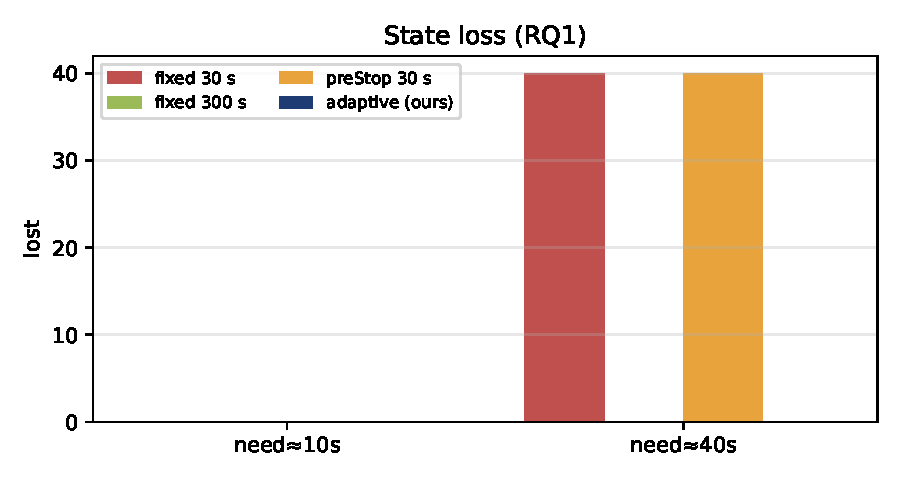
\includegraphics[width=\linewidth]{eval_state_loss.pdf}
    \caption{State loss (RQ1).}\label{fig:eval-loss}
  \end{subfigure}\hfill
  \begin{subfigure}[t]{0.49\linewidth}
    \centering
    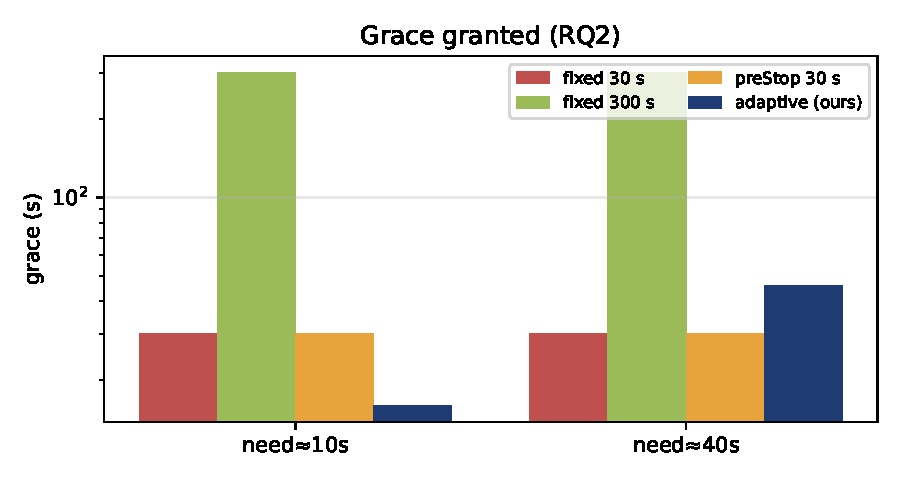
\includegraphics[width=\linewidth]{eval_grace_budget.pdf}
    \caption{Grace granted, log scale (RQ2).}\label{fig:eval-grace}
  \end{subfigure}
  \caption{Measured results. (\subref{fig:eval-loss})~Only the fixed-grace policies lose state, and
  only once the handoff outlasts the grace (heavy load). (\subref{fig:eval-grace})~The controller
  grants grace proportional to the need, while the over-provisioned baseline reserves a fixed
  300\,s.}\label{fig:eval}
\end{figure}

\paragraph{RQ1 (correctness).} Under heavy load the fixed 30\,s grace and the fixed \texttt{preStop}
sleep each lose \emph{40 of 160} processes: \texttt{SIGKILL} truncates the handoff at 30\,s while
$\approx$10\,s of work remains. The adaptive controller (grace 46\,s) and the over-provisioned 300\,s
grace lose none. Under light load, where the need is below the grace, every policy is loss-free.
A fixed grace is therefore unsafe exactly when the handoff outlasts it, and the controller removes
that loss by sizing the grace to the need.

\paragraph{RQ2 (efficiency).} The controller grants only the grace required---16\,s at light load and
46\,s at heavy load---whereas the over-provisioned baseline reserves a fixed 300\,s regardless: about
$18.8\times$ and $6.5\times$ the grace actually needed. A fixed-large grace matches the controller's
safety only by reserving a worst-case budget that bounds rollout pacing far above the real need.

\paragraph{RQ3 (adaptivity).} As the load rose (need $10\to40$\,s) the granted grace rose
$16\to46$\,s, tracking $|H|/\rho$ plus the safety margin. Every adaptive drain completed (drain time
$\approx$ need, zero loss) within the bound $g_{\max}$---no deadlock and no zombie pods.

\paragraph{Sweep across load (RQ1, RQ2).} Figure~\ref{fig:sweep} repeats the comparison over the
need sweep. The two fixed-grace policies lose no state while the need stays below the 30\,s grace,
then lose $\approx$103 of 400 processes once it exceeds it; the adaptive controller and the 300\,s
grace never lose state. The controller's granted grace tracks the need ($16\to31\to46$\,s for need
$10\to25\to40$\,s) while the fixed 300\,s reserves an order of magnitude more than required. Variance
over the three repeats is negligible---the mechanism is deterministic under the throttle.

\paragraph{Invariant validation (RQ1).} Figure~\ref{fig:invariant} plots, for every sweep point, the
granted grace against the handoff need and the safety floor $g=|H|/\rho$ of
Equation~\eqref{eq:invariant}. The adaptive controller sits just above the floor at every load (a
constant $\sigma$-margin), so the invariant---and hence Proposition~\ref{prop:safety}---holds
empirically across the sweep; the fixed 30\,s and \texttt{preStop} policies cross \emph{below} the
floor once the need exceeds 30\,s, landing in the unsafe region where the handoff is truncated (the
lost points, ringed). The fixed 300\,s policy is safe but sits far above the floor---reserving
roughly $6$--$7\times$ the grace the heaviest load needs, and an order of magnitude more under light
load. The controller is the only policy in the desirable region: above the floor (safe) yet close to
it (no over-provisioning).

\begin{figure}[t]
  \centering
  \begin{subfigure}[t]{0.49\linewidth}
    \centering
    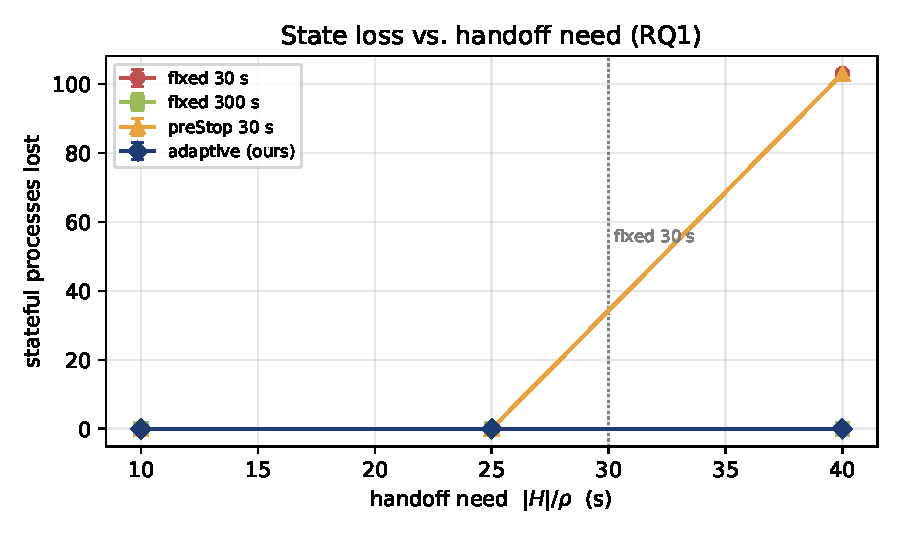
\includegraphics[width=\linewidth]{eval_sweep_loss.pdf}
    \caption{State loss vs.\ need (RQ1).}\label{fig:sweep-loss}
  \end{subfigure}\hfill
  \begin{subfigure}[t]{0.49\linewidth}
    \centering
    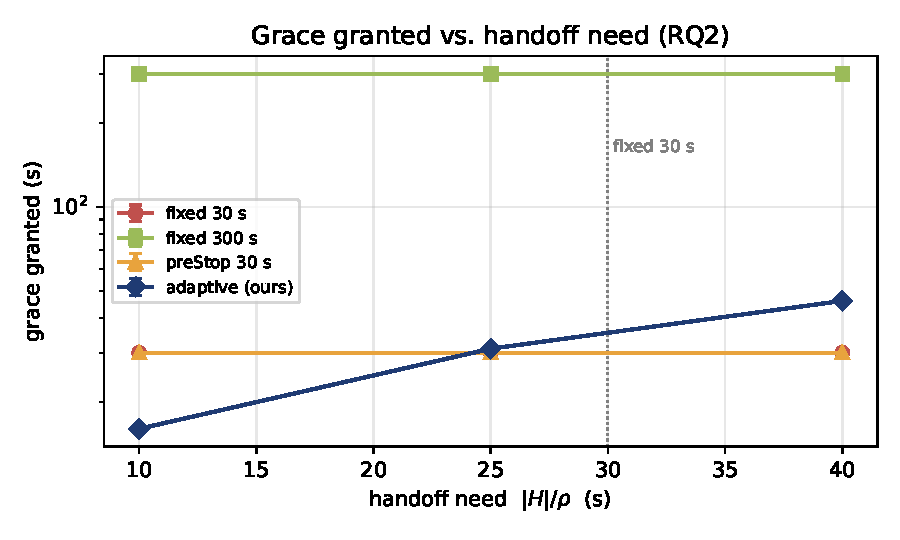
\includegraphics[width=\linewidth]{eval_sweep_grace.pdf}
    \caption{Grace granted vs.\ need (RQ2).}\label{fig:sweep-grace}
  \end{subfigure}
  \caption{Sweep over the handoff need (three repeats; the dotted line marks the 30\,s fixed grace).
  (\subref{fig:sweep-loss})~Fixed-grace policies lose state once the need crosses 30\,s;
  (\subref{fig:sweep-grace})~the controller stays loss-free and sizes the grace to the need.}\label{fig:sweep}
\end{figure}

\begin{figure}[t]
  \centering
  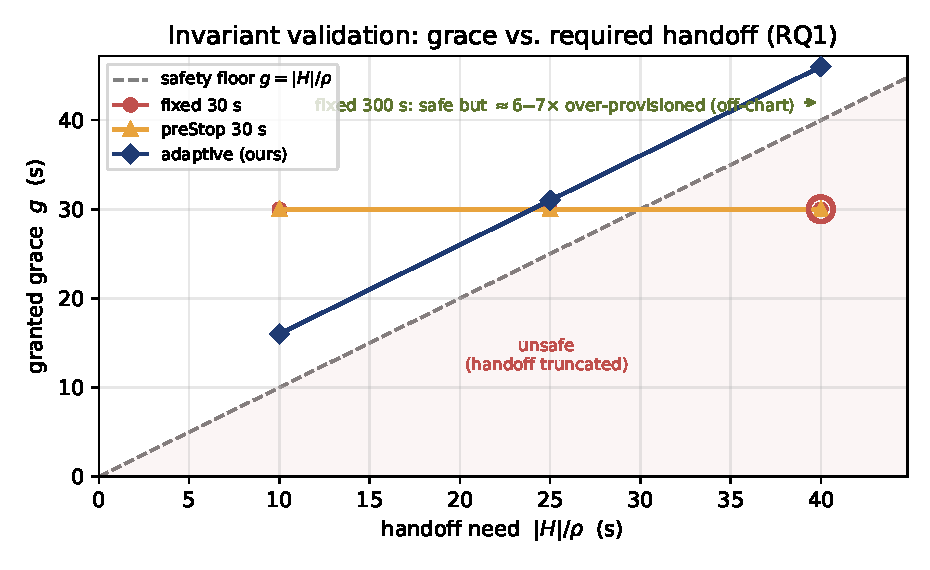
\includegraphics[width=0.82\linewidth]{eval_invariant.pdf}
  \caption{Granted grace versus required handoff. Points on or above the dashed safety floor
  $g=|H|/\rho$ satisfy the invariant (Equation~\eqref{eq:invariant}); the adaptive controller tracks
  it tightly, the fixed 30\,s and \texttt{preStop} policies fall into the unsafe region beyond a 30\,s
  need (ringed $=$ state lost), and the fixed 300\,s baseline (off-chart) is safe but heavily
  over-provisioned.}\label{fig:invariant}
\end{figure}

\paragraph{End-to-end rollout time (RQ2).} Figure~\ref{fig:rollout} times a three-pod rolling update
at need~$\approx$40\,s. The fixed 30\,s grace finishes fastest (90.6\,s) but loses 309 processes; the
over-provisioned 300\,s grace and the adaptive controller both complete in 121.9\,s with zero loss.
The controller thus matches the safe baseline's rollout time \emph{without} reserving its worst-case
budget---it pays only for the handoff that actually occurs.

\begin{figure}[t]
  \centering
  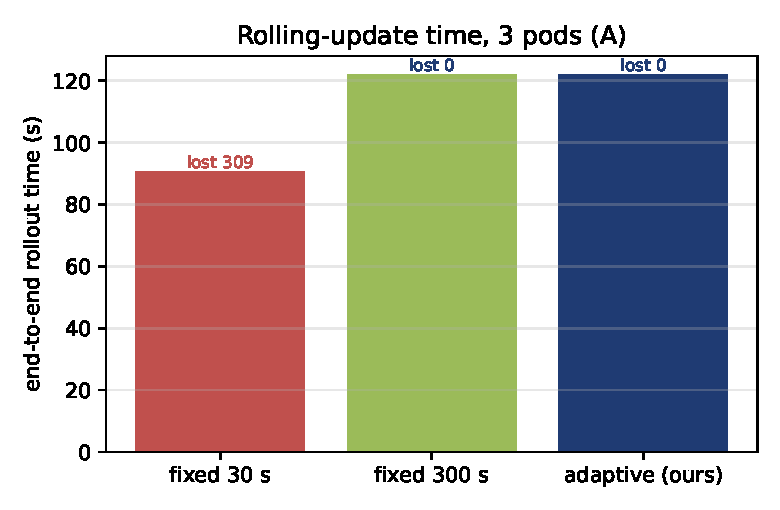
\includegraphics[width=0.6\linewidth]{eval_rollout.pdf}
  \caption{Rolling-update time for three pods at need~$\approx$40\,s. The fixed 30\,s grace is faster
  only because it abandons 309 in-flight processes.}\label{fig:rollout}
\end{figure}

\paragraph{Overhead (RQ4).} The controller is cheap. A probe reading costs $\approx 7\,\mu$s; each
stateful process adds $\approx 6.7$\,KB; and handoff sustains $\approx 8{,}300$ state transfers per
second unthrottled. On Kubernetes the operator's resident footprint is $\approx 73$\,MiB (dominated
by the BEAM VM), and one reconcile cycle---list pods, read every probe, compute, and patch the
Deployment---takes $\approx 74$\,ms every 5\,s, under 2\% duty. The mechanism's cost is negligible
against the state it preserves.

\paragraph{Robustness (RQ5).} Figure~\ref{fig:sens} varies the policy's inputs. The granted grace
rises linearly with the safety margin $\sigma$ ($21\to36$\,s for $\sigma=0\to15$) and is strictly
capped by $g_{\max}$ (clamped to 30/60/120\,s; the uncapped value of 206\,s appears only at
$g_{\max}=300$). The dominant lever is the rate estimate: under-estimating $\rho$ inflates the grace
(46\,s at $0.5\times$, conservative and safe), while over-estimating it shrinks the grace (16\,s at
$2\times$, risking truncation). The estimate should therefore be biased downward---which the
default-safe fallback (Section~\ref{sec:design-failsafe}) enforces when no rate is observed.

\begin{figure}[t]
  \centering
  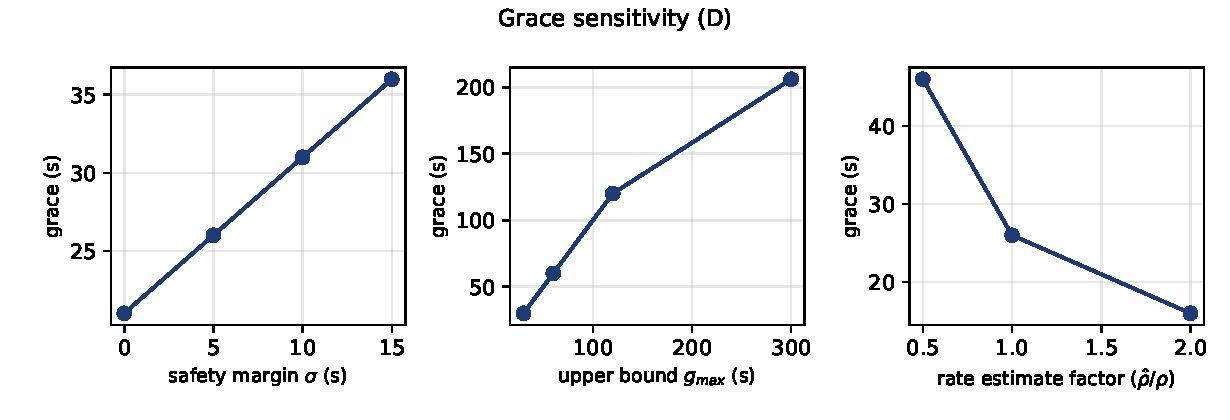
\includegraphics[width=\linewidth]{eval_sensitivity.pdf}
  \caption{Grace sensitivity: linear in the margin $\sigma$, capped by $g_{\max}$, and monotone in
  the rate estimate (bias it low to stay safe).}\label{fig:sens}
\end{figure}

The raw measurements are in the artifact (\texttt{data/results\_runs.csv}), regenerated by the
experiment harness (\texttt{harness/run.exs}).

\paragraph{Scalability (RQ6).} Figure~\ref{fig:scale} drives a single draining node from
$|H|=1{,}000$ to $40{,}000$ stateful processes, handing the entire backlog to one survivor
unthrottled. The two costs scale very differently. Memory grows \emph{linearly} and stays
modest---6 to 167\,MiB across the range ($\approx$4\,KB per process)---so RAM is not the binding
constraint. Handoff throughput, by contrast, \emph{degrades super-linearly}: it falls from
$\approx$3{,}000 transfers/s at $|H|=1{,}000$ to 123/s at $20{,}000$ and 67/s at $40{,}000$, because
every migration registers and resolves an identity in the cluster-wide delta-CRDT registry, whose
per-operation cost grows with the number of live entries. The result is a per-node ceiling: through
$|H|=20{,}000$ the node drains completely with zero loss (163\,s), but at $40{,}000$ it cannot finish
within a 600\,s budget and abandons $19{,}392$ of $40{,}000$ processes. This ceiling is a property of
the \emph{handoff substrate}---Horde's registry---not of the controller, whose grace computation is
constant-time and whose granted grace rises monotonically (7 to 46\,s) as throughput drops. It does,
however, expose a limit of any rate-based policy: the linear model $|H|/\rho$ assumes a stable $\rho$,
yet at extreme backlogs the effective throughput collapses, so a single-snapshot rate
under-predicts the true handoff time---reinforcing RQ5's guidance to estimate $\rho$ conservatively.
The operational remedy is the same either way: bound the per-pod stateful backlog and scale
\emph{horizontally} (more replicas, smaller $|H|$ each), which the Kubernetes deployment supports
directly; raising the per-node ceiling by sharding the registry is future work. Raw data is in
\texttt{data/results\_scale.csv} (harness \texttt{harness/scale.exs}).

\begin{figure}[t]
  \centering
  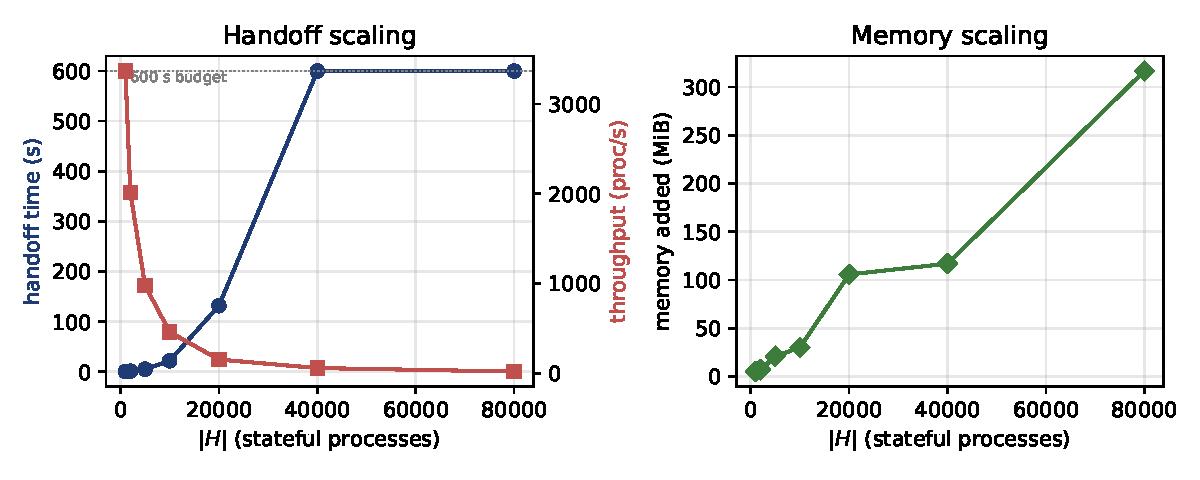
\includegraphics[width=\linewidth]{eval_scale.pdf}
  \caption{Per-node handoff scaling. Memory grows linearly (right), but handoff throughput collapses
  super-linearly as the delta-CRDT registry fills (left), capping the backlog a single pod can drain
  within a fixed budget. At $|H|=40{,}000$ the 600\,s drain budget expires with $19{,}392$ processes
  un-migrated.}\label{fig:scale}
\end{figure}

\paragraph{Kubernetes deployment.} We also deployed the full artifact on a Kubernetes cluster
(\texttt{kind}): the service as a three-replica Deployment that forms a BEAM cluster through the
libcluster Kubernetes strategy, the coordinator as a separate operator Deployment, and the adaptive
\texttt{preStop} hook on each pod. End-to-end, the operator read every pod's probe and patched the
Deployment's \texttt{terminationGracePeriodSeconds} from the runtime backlog---raising it from 6\,s
when idle to 26\,s once roughly 190 stateful processes per pod had accumulated at a 10/s handoff
rate---confirming the cross-layer feedback loop on a real orchestrator. The quantitative loss and
efficiency figures above come from the controlled BEAM-cluster experiment; this run validates the
deployment artifacts and the operator's control loop.

\paragraph{Network-latency realism (RQ7).} Our controlled measurements run on a single host, where
inter-node transfer is near-instant; a reviewer-critical question is whether the rate signal $\rho$
that drives the policy reflects \emph{real} network latency. We tested this directly on the
\texttt{kind} cluster by injecting per-packet delay with \texttt{tc netem} on the survivor pods'
egress and measuring, from a leaving pod, the inter-pod round-trip time of the synchronous handoff
RPC (Figure~\ref{fig:netem}; harness \texttt{k8s/netem.sh}). The measured RTT tracks the injected
delay to within $0.3$\,ms, confirming the latency is real and on the handoff path. Because each state
transfer is one such round-trip, the achievable rate $\rho\approx 1/\mathrm{RTT}$ collapses from
$\approx$23{,}800\,proc/s at sub-millisecond RTT to $19.9$, $9.8$, and $6.7$\,proc/s at $50$, $100$,
and $150$\,ms. The controller responds correctly: the grace it would grant a representative
$2{,}000$-process backlog rises from the floor ($6$\,s) to $107$\,s at $50$\,ms RTT, then saturates
the $g_{\max}=120$\,s cap beyond $100$\,ms. This validates that $\rho$ captures genuine network
cost---so the single-host efficiency numbers are conservative rather than optimistic---and pinpoints,
for a given $g_{\max}$, the latency past which a pod's backlog must shrink or the cap must rise:
exactly hypothesis~(ii) of Proposition~\ref{prop:safety}.

\begin{figure}[t]
  \centering
  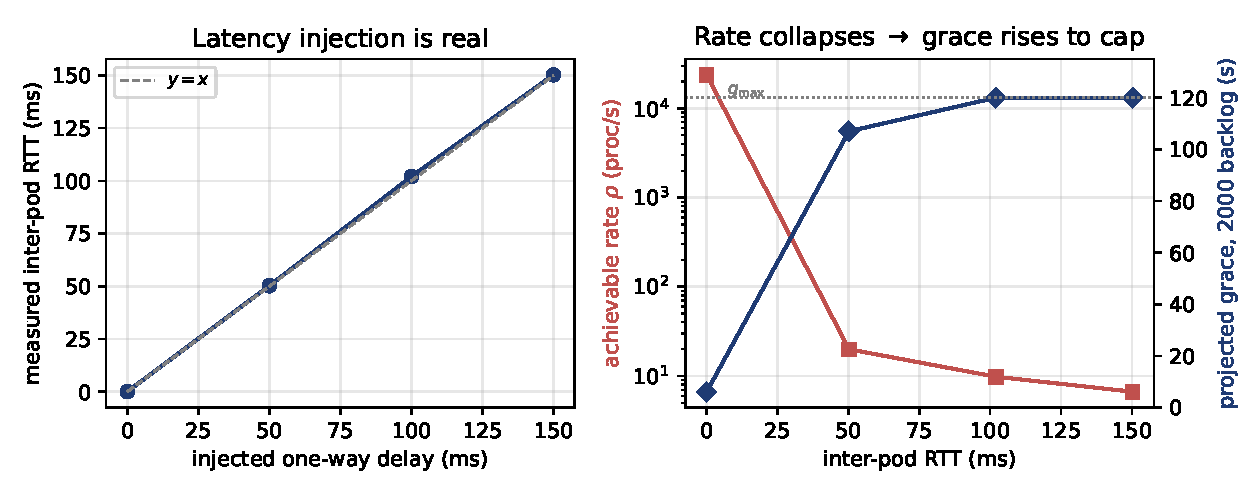
\includegraphics[width=\linewidth]{eval_netem.pdf}
  \caption{Real inter-pod latency injected with \texttt{tc netem} on the \texttt{kind} cluster.
  Left: measured RTT tracks the injected delay ($y=x$), so the latency is real and on the handoff
  path. Right: the achievable handoff rate $\rho\approx1/\mathrm{RTT}$ collapses (log scale) and the
  grace the policy grants a $2{,}000$-process backlog rises until it saturates $g_{\max}$ beyond
  $\approx$100\,ms RTT.}\label{fig:netem}
\end{figure}

\paragraph{Fail-safe validation.} Section~\ref{sec:design-failsafe} claims the controller degrades
safely; we injected three faults on the live cluster to check (harness \texttt{k8s/faults.sh},
Table~\ref{tab:faults}). Killing the coordinator pod cost no safety: a fresh operator recovered,
re-read the probes, and re-patched the same grace---assignment is idempotent. Feeding the policy an
unusable probe (a positive backlog with a zero or missing rate) returned the configured fallback
($g_{\max}=120$\,s)---the \emph{largest} safe grace, never a small one. Revoking the operator's API
permissions mid-operation produced no crash loop (zero restarts) and left the last grace in place: a
controller that cannot reach the API server stops updating rather than driving the grace to an unsafe
value. In all three cases the failure mode is conservative, matching the design.

\begin{table}[t]
\centering
\caption{Fail-safe validation on the live cluster: injected faults and the controller's
conservative response.}\label{tab:faults}
\begin{tabular}{@{}lll@{}}
\toprule
\textbf{Injected fault} & \textbf{Response} & \textbf{Outcome} \\
\midrule
Coordinator pod killed & restart, re-probe, re-patch & recovered; grace stable ($6\!\to\!6$\,s) \\
Probe unusable (rate $0$/missing) & return fallback & grace $=g_{\max}$ ($120$\,s), default-safe \\
API permission revoked & error caught, no patch & no crash ($0$ restarts); last grace persists \\
\bottomrule
\end{tabular}
\end{table}

\paragraph{Realistic-workload case study: Phoenix.Presence (RQ8).} To check the mechanism on a real,
unmodified distributed feature rather than synthetic workers, we exercise \texttt{Phoenix.Tracker}---
the CRDT engine behind \texttt{Phoenix.Presence}, widely used to track who-is-online across a
cluster. We track $N$ presences on the leaving node and, on a graceful departure, measure how long
the survivor takes to re-converge---the $T_c$ term of Equation~\eqref{eq:invariant}
(Figure~\ref{fig:presence}; harness \texttt{harness/presence.exs}). Re-convergence is $\approx$1.5\,s
and, unlike handoff, essentially \emph{independent of $N$} (100 to 2{,}000 presences), because it is
paced by the tracker's CRDT broadcast period, not the presence count; add-convergence is faster
($0.3$--$0.7$\,s). Two things follow. First, the coupling holds on a real workload: $T_c$ is a
bounded, measurable quantity the grace must cover, and the controller already includes it. Second,
the measured $\approx$1.5\,s is roughly $30\times$ our deliberately crude built-in estimate
($50$\,ms per peer); the default margin $\sigma=5$\,s absorbs the gap, but a production deployment
should feed a \emph{measured} convergence signal into the probe rather than the heuristic---an honest
limitation this case study exposes.

\begin{figure}[t]
  \centering
  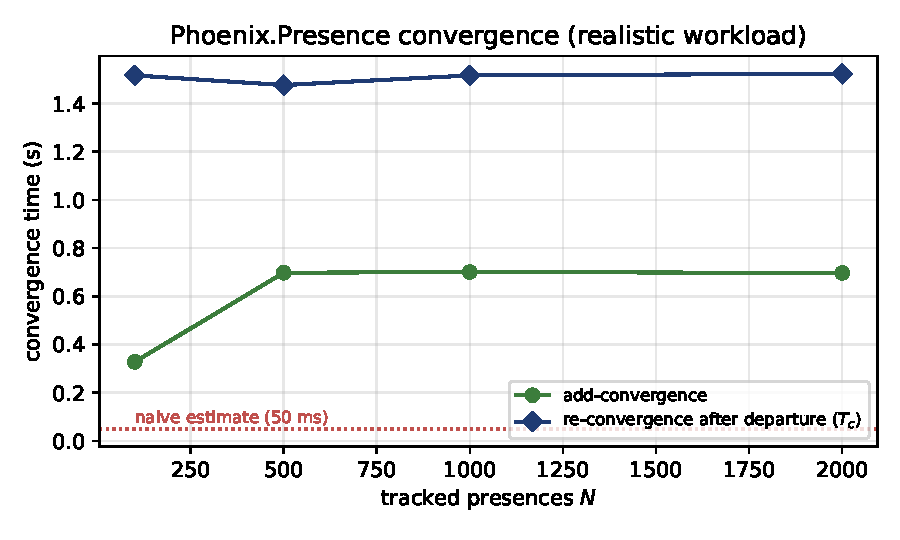
\includegraphics[width=0.78\linewidth]{eval_presence.pdf}
  \caption{Realistic workload: \texttt{Phoenix.Tracker}/\texttt{Presence} convergence on a graceful
  node departure. Re-convergence ($T_c$) is $\approx$1.5\,s and nearly independent of the
  tracked-presence count $N$ (it is set by the CRDT broadcast period), about $30\times$ the naive
  50\,ms estimate; the safety margin $\sigma$ covers it.}\label{fig:presence}
\end{figure}

%====================================================================
\section{Discussion and Threats to Validity}\label{sec:discuss}
\paragraph{Emulated cluster.} Our measurements come from a two-node cluster on a single host, not a
multi-machine deployment; the node count and host topology are emulated. The mechanism is
host-count-agnostic---the controller reads per-pod runtime signals and sets a per-pod grace---so we
expect the trend to hold on a real cluster, but a multi-machine (or cloud) confirmation run remains
future work; the Kubernetes deployment (Section~\ref{sec:eval}) likewise ran on a single-host
\texttt{kind} cluster. We partly close this gap by injecting \emph{real} inter-pod network latency
with \texttt{tc netem} (RQ7, Figure~\ref{fig:netem}): the rate signal tracks the injected RTT, so the
single-host efficiency numbers are conservative---a real network only lowers $\rho$, which the
controller already compensates for by granting more grace.

\paragraph{Rate estimation.} The controller sizes the grace from the handoff rate $\rho$. In our
experiments $\rho$ is the known achievable transfer throughput; in production it is estimated online
(an EWMA of observed handoffs). A lagging estimate under bursty load is bounded on both sides: the
margin $\sigma$ and the bounds $g_{\min},g_{\max}$ cap the error, and an unavailable or implausible
reading triggers the default-safe fallback (Section~\ref{sec:design-failsafe}). A further limit
surfaces at extreme backlogs (RQ6): because the handoff substrate's throughput collapses
super-linearly, a single-snapshot $\rho$ over-estimates the achievable rate and the policy can
under-provision grace---so $\rho$ should be biased conservatively and per-pod backlog bounded.

\paragraph{Per-node handoff ceiling.} Scalability (RQ6, Figure~\ref{fig:scale}) is bounded not by
the controller---whose grace computation is constant-time---but by the cluster-wide registry: its
per-operation cost grows with the number of live entries, so a single node's handoff throughput
degrades super-linearly and a pod holding tens of thousands of stateful processes cannot drain
within a practical grace window. We mitigate this operationally by bounding per-pod backlog and
scaling horizontally; removing it at the substrate level (e.g., a sharded or partitioned registry)
is future work and orthogonal to the cross-layer coupling this paper contributes.

\paragraph{Scope.} The controller addresses \emph{voluntary} disruptions (rolling updates, drains,
scale-down), where a grace window exists. Abrupt, non-graceful node death gives no window and loses
unmigrated state regardless of policy; tolerating it needs replication or checkpointing, which is
orthogonal and out of scope.

\paragraph{Measurement.} The headline scenarios (Table~\ref{tab:eval}) are each repeated 10 times:
loss and grace are exactly reproducible and drain time varies by $<0.01$\,s (95\% CI $\le\pm0.003$\,s),
confirming the determinism the throttle induces---variance is not a confound here. Rolling-update
times are likewise reproducible across repeats (\texttt{data/results\_rollout\_ci.csv}). We evaluate
one realisation (BEAM); the principle's generality to other runtimes is argued qualitatively
(Section~\ref{sec:related}), not benchmarked.

\subsection{Practitioner guidance}\label{sec:guidance}
Our findings translate into concrete advice for operators running stateful services on Kubernetes.
\begin{itemize}
  \item \textbf{Size the grace from a runtime signal, not a guess.} A constant is wrong in both
  directions---unsafe when handoff outlasts it, wasteful when it does not. Until a controller is in
  place, prefer over-provisioning to under-provisioning: lost state is irreversible, extra latency is
  not.
  \item \textbf{Bound the per-pod stateful backlog.} Handoff cost grows super-linearly in $|H|$
  (RQ6); keep $|H|$ below the point where the handoff fits the grace, and scale out (more replicas,
  smaller $|H|$) rather than up.
  \item \textbf{Bias the rate estimate low.} Under-estimating $\rho$ inflates the grace (safe);
  over-estimating truncates the handoff (RQ5, RQ7). The default-safe fallback enforces this when no
  rate is observed.
  \item \textbf{Set $g_{\max}$ from the latency budget.} At inter-pod RTT $R$, a backlog $B$ needs
  $\approx B/\rho(R)$ seconds (RQ7); choose $g_{\max}$ to cover the worst expected $(B,R)$, or cap
  $B$ so the need stays below $g_{\max}$.
  \item \textbf{Spend the grace draining, not sleeping.} A \texttt{preStop} that finishes handoff and
  returns early beats a fixed sleep---both safer and faster.
  \item \textbf{Make the loop default-safe and idempotent.} Fall back to the maximum grace on missing
  signals, and keep grace assignment idempotent so a coordinator restart cannot corrupt an in-flight
  rollout (Table~\ref{tab:faults}).
\end{itemize}

%====================================================================
\section{Related Work}\label{sec:related}
% Position M3 vs: dependable microservices in K8s (JISA 2024), RTilience (TSC
% 2025), Istio resilience (Cluster Computing 2025), proactive stateful lifecycle
% (Computer Communications 2025), eBPF-Shield (SOCA 2025/26), Akka Lease/SBR,
% Glasgow SCM, Nefele. None tie grace to runtime convergence signals -> the gap.

Most cloud-native resilience work treats the orchestrator and the application runtime as separate
concerns. Chaos-engineering and practitioner studies inject faults and survey recovery in Kubernetes
microservices~\cite{singh2025istio,souza2024dependable}; proactive lifecycle managers migrate
stateful microservices across clusters~\cite{meliani2025proactive}; deployment-time planners place
components under fault-tolerance and latency constraints~\cite{ucc23,gustafsson2025rtilience}; and
signal-based health monitoring derives a pod's Kubernetes health from runtime state instead of
polling it~\cite{roberts2025}. These cross the orchestrator/runtime boundary for \emph{health},
\emph{placement}, or \emph{recovery}, yet none couples the termination grace period to the runtime's
handoff and convergence progress---the specific feedback our controller adds.

\subsection{Graceful shutdown in other actor runtimes}\label{sec:related-actors}
% Use the ROLE vocabulary of Table~\ref{tab:roles} so the comparison is about
% responsibilities, not product names. The point: peer runtimes already provide a
% graceful-shutdown ROLE, but none DERIVE the orchestrator grace period from runtime
% convergence signals -- they use configured/static timeouts. That is M3's gap.

Other actor runtimes already provide a graceful-shutdown role. Akka's
\emph{CoordinatedShutdown} runs ordered shutdown phases with per-phase
timeouts~\cite{akkacoordinated}; Orleans performs graceful silo shutdown with grain
deactivation~\cite{orleans}. In both, however, the timeouts are \emph{configured
constants}, internal to the runtime, and are not fed back to the orchestrator's
termination grace period---so the same grace gap we target can occur. Our controller differs by
closing an explicit cross-layer feedback loop: the grace period is \emph{derived} at
run time from convergence signals (handoff backlog, observed rate $\rho$, membership
convergence) rather than guessed ahead of time (Table~\ref{tab:actor-compare}).
A multi-runtime implementation is left to future work; here we evaluate the BEAM
realisation and compare the others qualitatively.

\begin{table}[t]
\centering
\caption{Graceful shutdown across actor runtimes, by role. Peers provide a
shutdown role but use configured/static timeouts; only our controller derives the orchestrator
grace period from runtime convergence signals.}\label{tab:actor-compare}
\begin{tabular}{@{}p{0.26\linewidth}p{0.34\linewidth}p{0.15\linewidth}p{0.15\linewidth}@{}}
\toprule
\textbf{Runtime} & \textbf{Shutdown mechanism} & \textbf{Cross-layer coupling} & \textbf{Grace from convergence?} \\
\midrule
BEAM + Kubernetes (common practice) & preStop hook + static \texttt{terminationGracePeriodSeconds} & manual / static & No \\
Akka & CoordinatedShutdown (phased, per-phase timeouts) & partial (runtime-internal) & No \\
Orleans & graceful silo shutdown / grain deactivation & partial (runtime-internal) & No \\
\textbf{This paper} & adaptive grace-convergence controller & \textbf{explicit feedback} & \textbf{Yes} \\
\bottomrule
\end{tabular}
\end{table}

%====================================================================
\section{Conclusion}\label{sec:conc}
A fixed termination grace period is structurally mismatched to stateful handoff: the orchestrator
fixes the deadline while the runtime holds the information that should set it. We presented a
cross-layer controller that derives the grace period at run time from the runtime's handoff and
convergence signals and paces the rolling update accordingly, realised as an open artifact on
Elixir/OTP with Horde, libcluster, and a Kubernetes operator. We proved the policy satisfies the
grace-safety invariant under a conservative rate estimate, and the implementation bears this out: on a
two-node cluster it eliminated the state loss a fixed 30\,s grace incurs once the handoff outlasts it
(40 of 160 processes), while granting only the grace actually needed (16--46\,s) instead of a fixed,
over-provisioned 300\,s. Repeated runs were deterministic; injecting real inter-pod latency confirmed
the controller tracks genuine handoff cost; a scalability sweep located the per-node handoff ceiling
that bounds a single pod's backlog; and fault injection confirmed the controller degrades safely.
Future work scales the Kubernetes deployment to multiple machines and production workloads,
generalises the principle to other actor runtimes, and pursues the broader cross-layer agenda---coordinating disruption budgets
with cluster quorum, compiling a single deployment specification to both layers, and aligning
restart budgets with backoff.

%====================================================================
\appendix

\section{Reproducing the results}\label{app:repro}
The artifact (\texttt{code/}) regenerates every number and figure in this paper. All commands run from
\texttt{code/app} unless noted; the distributed experiments spawn a survivor peer, so they need a
named node.

\paragraph{Tests.} \texttt{mix deps.get \&\& mix test} runs the 6 policy unit tests; the two-node
cluster integration test (state-preserving handoff and truncation-under-short-grace) runs with
\texttt{MIX\_ENV=test elixir --name primary@127.0.0.1 --cookie ck -S mix test --only cluster}.

\paragraph{Controlled experiments (Tables~\ref{tab:eval}, \ref{tab:faults}; Figures~\ref{fig:eval}--\ref{fig:netem}).}
Drive each harness with the same named node, e.g.\
\texttt{... -S mix run harness/run.exs}. The harnesses are: \texttt{run.exs} (the two table loads),
\texttt{sweep.exs} (the load sweep, rolling update, overhead, and sensitivity), \texttt{repeats.exs}
(10 repeats for the confidence intervals), and \texttt{scale.exs} (the $|H|$ scalability sweep, RQ6).
Each writes a CSV under \texttt{data/}; \texttt{\textasciitilde/venv/bin/python analysis/plot.py} then
renders the figures into \texttt{figures/}.

\paragraph{Kubernetes (kind).} Build the image, create a cluster, and apply the manifests
(\texttt{kubectl apply -f code/k8s/}); the operator then patches the Deployment's grace from the live
backlog. The real-latency experiment (RQ7, Figure~\ref{fig:netem}) is \texttt{bash code/k8s/netem.sh};
the fail-safe injection (Table~\ref{tab:faults}) is \texttt{bash code/k8s/faults.sh}.

\section{Additional listings}\label{app:manifests}
Listing~\ref{lst:drain} is the handoff drain loop referenced in Section~\ref{sec:impl-handoff}: it
transfers local workers one at a time until the backlog clears or the deadline (the granted grace)
elapses---the latter being exactly the truncated handoff a too-short grace produces. Listing~\ref{lst:rbac}
gives the Kubernetes objects omitted from Section~\ref{sec:impl-pack}: the headless Service for BEAM
discovery, the PodDisruptionBudget, and the operator's least-privilege RBAC.

\begin{lstlisting}[language=Elixir, caption={The handoff drain loop (\texttt{Handoff.drain/2}): hand off until the backlog clears or the deadline elapses.}, label=lst:drain]
defp loop(deadline, rate_limit) do
  cond do
    Workers.local_count() == 0 -> :ok
    now_ms() >= deadline -> {:timeout, Workers.local_count()}   # grace expired: state lost
    true ->
      case Workers.local() do
        [{id, pid} | _] ->
          case handoff_one(id, pid) do                          # read state, stop local, place on survivor
            :ok -> if rate_limit, do: Process.sleep(max(1, trunc(1000 / rate_limit)))
            :no_survivor -> Process.sleep(100)
          end
          loop(deadline, rate_limit)
        [] -> :ok
      end
  end
end
\end{lstlisting}

\begin{lstlisting}[caption={Discovery, disruption budget, and operator RBAC (abridged).}, label=lst:rbac]
# headless Service: per-pod DNS for BEAM distribution
kind: Service
spec: { clusterIP: None, selector: { app: grace }, ports: [ {name: epmd, port: 4369} ] }
---
kind: PodDisruptionBudget
spec: { maxUnavailable: 1, selector: { matchLabels: { app: grace } } }
---
kind: Role            # operator: read pods, patch the Deployment's grace
rules:
  - { apiGroups: [""],     resources: ["pods"],        verbs: ["get","list"] }
  - { apiGroups: ["apps"], resources: ["deployments"], verbs: ["get","list","patch"] }
\end{lstlisting}

\bibliography{references}

\end{document}
